%% 
%% Copyright 2019-2020 Elsevier Ltd
%% 
%% This file is part of the 'CAS Bundle'.
%% --------------------------------------
%% 
%% It may be distributed under the conditions of the LaTeX Project Public
%% License, either version 1.2 of this license or (at your option) any
%% later version. The latest version of this license is in
%%    http://www.latex-project.org/lppl.txt
%% and version 1.2 or later is part of all distributions of LaTeX
%% version 1999/12/01 or later.
%% 
%% The list of all files belonging to the 'CAS Bundle' is
%% given in the file `manifest.txt'.
%% 
%% Template article for cas-sc documentclass for 
%% double column output.

%\documentclass[a4paper,fleqn,longmktitle]{cas-sc}
\documentclass[a4paper,fleqn]{cas-sc}

% \usepackage[numbers]{natbib}
%\usepackage[authoryear]{natbib}
\usepackage[authoryear,longnamesfirst]{natbib}
\usepackage{amsmath}
\usepackage{tcolorbox}
\tcbuselibrary{theorems}
\usepackage{graphicx}
\usepackage{subcaption}
% \usepackage{wrapfig}

\usepackage{placeins}
\usepackage{threeparttable}
\usepackage{booktabs}
\usepackage{caption}
\usepackage{float}
\usepackage{tikz}
\usetikzlibrary{
    arrows.meta,
    positioning,
    shapes.geometric,
    shapes.misc,
    fit,
    backgrounds
}


%%%Author definitions
\def\tsc#1{\csdef{#1}{\textsc{\lowercase{#1}}\xspace}}
\tsc{WGM}
\tsc{QE}
\tsc{EP}
\tsc{PMS}
\tsc{BEC}
\tsc{DE}
%%%

% Uncomment and use as needed
%\newtheorem{theorem}{Theorem}
%\newtheorem{lemma}[theorem]{Lemma}
%\newdefinition{rmk}{Remark}
%\newproof{pf}{Proof}
%\newproof{pot}{Proof of Theorem \ref{thm}}

\begin{document}
\let\WriteBookmarks\relax
\renewcommand{\topfraction}{0.85}
\renewcommand{\bottomfraction}{0.85}
\renewcommand{\textfraction}{0.10}
\renewcommand{\floatpagefraction}{0.75}

% Short title
\shorttitle{Mobile Money Fraud Detection}

% Short author
\shortauthors{ Ongaro,M.}

% Main title of the paper
\title [mode = title]{SAAB-DL: Overcoming Extreme Class Imbalance in Mobile Money Fraud Detection via Deep Behavioural and Structural Embeddings}                      
% Title footnote mark
% eg: \tnotemark[1]
\tnotemark[1,2]

% Title footnote 1.
% eg: \tnotetext[1]{Title footnote text}
% \tnotetext[<tnote number>]{<tnote text>} 



% First author
%
% Options: Use if required
% eg: \author[1,3]{Author Name}[type=editor,
%       style=chinese,
%       auid=000,
%       bioid=1,
%       prefix=Sir,
%       orcid=0000-0000-0000-0000,
%       facebook=<facebook id>,
%       twitter=<twitter id>,
%       linkedin=<linkedin id>,
%       gplus=<gplus id>]
\author[1]{David Ongaro M.E}[type=editor,
                        auid=000,bioid=1,
                        prefix=Mr,
                        role=Researcher]
% Corresponding author indication

% Footnote of the first author
\fnmark[1]

% Email ID of the first author
\ead{david.mauti@strathmore.edu}

% URL of the first author
% \ead[url]{www.cvr.cc, cvr@sayahna.org}

%  Credit authorship
% \credit{Conceptualisation of this study, Methodology, Software}

% Address/affiliation
\affiliation[3]{organization={Strathmore University},
    addressline={Ole Sangale}, 
    city={Nairobi},
    % citysep={}, % Uncomment if no comma needed between city and postcode
    state={Nairobi},
    country={Kenya}}


% For a title note without a number/mark


% Here goes the abstract
\begin{abstract}
The rapid expansion of mobile money ecosystems in emerging markets has driven financial inclusion but concurrently expanded the attack surface for complex financial fraud. A primary challenge in detecting such fraud is the extreme class imbalance inherent in transaction logs. This study addresses the problem of detecting mobile money fraud in highly imbalanced environments by transitioning from traditional linear models to advanced, nonlinear architectures capable of capturing both behavioural and structural anomalies. The research utilises a dataset of 95,662 anonymised transactions from an East African mobile money provider, analysed using the CRISP-DM framework. Key Exploratory Data Analysis (EDA) approaches included evaluating class distributions, analysing transaction value disparities, and assessing temporal patterns. To address the imbalance, the study deployed and compared five baseline machine learning algorithms against a novel framework: SMOTE-Aware Adaptive Boosting with Deep Learning (SAAB-DL). This novel approach fuses Variational Autoencoder (VAE) behavioural embeddings with Graph Neural Network (GNN) structural topologies into a unified feature space, utilising Local Density Scoring to guide conditional synthetic augmentation. EDA confirmed a severe 0.202\% fraud prevalence and revealed that fraud cases typically involve significantly higher transaction amounts and distinct temporal clustering. Machine learning results demonstrated that tree-based gradient boosting models, specifically LightGBM utilising cost-sensitive learning, substantially outperformed linear models, which failed to capture the nonlinear fraud manifolds. The proposed SAAB-DL framework achieved an exceptional Precision-Recall AUC (PR-AUC) of 0.9296 and an F1-score of 0.8800 on the primary evaluation set, and maintained a highly robust mean F1-score of 0.9420 across 18 rigorous stress-test scenarios. This demonstrates that its modular integration of deep feature extraction provides a highly discriminative representation for identifying fraud patterns. The optimised framework was successfully deployed as a real-time Streamlit prototype, validating its operational feasibility with millisecond-level inference latency. Ultimately, this study highlights that effective mobile money fraud detection requires algorithms that explicitly account for extreme imbalance, providing a data-driven blueprint for financial institutions globally to build scalable, adaptive defence mechanisms against evolving digital fraud vectors.
\end{abstract}

\maketitle

\section{Introduction}
The rapid adoption of digital financial solutions continues to redefine economic activity across many developing countries, with mobile money platforms serving as a cornerstone of financial inclusion. Worldwide, mobile money systems supported 1.75 billion registered accounts by end of 2023, with Sub-Saharan Africa accounting for the largest share of adoption \cite{GSMA_SOTIR_2024}. Despite these transformative benefits, the rapid expansion of mobile money ecosystems has substantially increased the attack surface for financial fraud, resulting in considerable economic losses and eroding platform trust \cite{Azamuke2025Financial}. In Kenya specifically, nearly 47.4\% of mobile money users reported experiencing a loss of money, primarily through phone fraud, in the year preceding the survey \cite{finaccess2021household}. Collectively, these figures underscore the urgency of developing robust, adaptive fraud detection mechanisms tailored to this context.

Detecting fraud in mobile money transactions poses challenges that differ markedly from those encountered in traditional banking systems \cite{Azamuke2025Financial}. A primary difficulty arises from extreme class imbalance, where fraudulent transactions constitute only a minuscule fraction of overall volume, constraining the practical utility of standard machine learning models in learning meaningful minority class boundaries \cite{imbalanced1}. In addition, fraudsters continually refine their methodologies, exploiting coordinated network structures to circumvent single-user controls \cite{George2023Systematic}. Modern payment infrastructures require almost instantaneous assessment of these compl

While classical ensemble methods, most notably Random Forests and Gradient Boosting Machines, have gained traction in transaction screening, they frequently struggle when faced with severe, noisy class imbalances in real-time settings \cite{frontiersfrai2025}. To compensate, researchers often rely on global synthetic oversampling techniques such as SMOTE \cite{Hanbali2025MobileMoneyFraud}. However, blindly generating synthetic data risks introducing noise into dense legitimate feature spaces, leading to degraded precision in production environments \cite{Bonde2025Improving}. Concurrently, emerging deep learning techniques such as Graph Neural Networks demonstrate distinct promise in mapping hidden relational anomalies among accounts \cite{cheng2025graph}, but are computationally intensive and rarely combined efficiently with cost-sensitive structural ensembles \cite{kungu2026hybrid}.

Against this backdrop, the primary contribution of this study is the development of a hybrid SMOTE-Aware Adaptive Boosting and Deep Learning (SAAB-DL) framework. Utilising the Cross-Industry Standard Process for Data Mining (CRISP-DM), this study isolates deep behavioural embeddings using a Variational Autoencoder (VAE) and structural embeddings using a Graph Neural Network (GNN). To overcome the limits of traditional imbalance strategies, we introduce a conditional synthetic augmentation layer guided by Local Density Scoring (kk
k-NN bounds), allowing our adaptive ensemble to learn dense fraud boundaries without sacrificing legitimate user precision. By systematically benchmarking SAAB-DL against existing baselines using real East African transaction data, this study provides a resilient, data-driven methodology for advancing operational mobile money fraud defence.


\section{Literature Review}

\subsection{Mobile Money and Fintech Security}

The proliferation of mobile money platforms across Sub-Saharan Africa has stimulated a growing body of empirical research targeting fraud detection in these context-specific financial ecosystems. \cite{botchey2020mobile} conducted a cross-case analysis comparing Support Vector Machines (SVMs), Gradient-Boosted Decision Trees (GBDTs), and Na\"ive Bayes classifiers across multiple mobile money datasets. While GBDTs achieved the highest F1-scores, the authors acknowledged that all models suffered from precision degradation when class imbalance exceeded 1:200. Additionally, the datasets used in the study were relatively small ($<$50,000 transactions), limiting external validity. In a subsequent study, \cite{botchey2022predicting} extended this analysis by evaluating the effects of SMOTE resampling on the same mobile money context. Their findings demonstrated that SMOTE improved recall for XGBoost from 0.71 to 0.84; however, precision simultaneously dropped by 12\%, revealing the synthetic noise trade-off that this study aims to mitigate.

\cite{Lokanan2023predicting} applied Random Forest, Logistic Regression, and Gradient Boosting to a multi-agent-based PaySim simulated corpus of 1,048,575 transactions, reporting ROC-AUC values above 0.92 for all models. Despite these figures, the study relied exclusively on ROC-AUC, which can be misleadingly optimistic under extreme class imbalance \cite{Saito2015PrecisionRecall}. The absence of PR-AUC or F1-based evaluation limits the practical reliability of these conclusions. Similarly, \cite{Azamuke2025Financial} utilised rich synthetic mobile money data to train ensemble classifiers, enabling continuous retraining evaluations that account for concept drift. However, the synthetic fidelity of such data relative to live production traffic remains contested.

A notable gap in the broader fraud detection literature is its predominant focus on credit card transaction datasets from developed economies. As Azamuke et al. \cite{Azamuke2025Financial} demonstrate in their Sub-Saharan African context, the fraudulent scenarios encountered on mobile money platforms differ substantially from those captured in standard credit card benchmarks, necessitating domain-specific datasets and detection approaches that incorporate local transaction patterns and infrastructure-specific latency constraints.

\subsection{Machine Learning and Deep Learning in Fraud Detection}

\subsubsection{Ensemble Learning Approaches}
Traditional machine learning techniques have historically served as the foundation for anomaly detection in financial settings. For instance, \cite{hajek2022fraud} developed an XGBoost-based framework for mobile payment fraud, achieving an F1-score of 0.89 on an e-commerce dataset of 600,000 transactions. The framework leveraged engineered velocity and frequency features; however, no deep feature extraction was employed, and the evaluation used a single train-test split without cross-validation, which may overestimate generalisation.

More recently, Gradient Boosting algorithms, specifically XGBoost, LightGBM, and CatBoost have superseded earlier classifiers due to their efficient tree construction and superior handling of sparse features. \cite{Theodorakopoulos2025BigData} implemented a PySpark-distributed framework benchmarking XGBoost and CatBoost on the Kaggle Credit Card Fraud Detection dataset — 284,807 European cardholder transactions with a fraud rate of 0.172\%  with XGBoost achieving 99.97\% accuracy and a Brier Score of 0.0002, and CatBoost demonstrating superior probabilistic calibration. However, the study reports no ROC-AUC metrics despite the severe class imbalance making calibration-aware evaluation essential. Additionally, their evaluation is further confined to a single static dataset with no treatment of temporal feature dynamics, and the highly anonymised PCA-derived features (V1-V28) preclude any meaningful feature interpretability or transferability to mobile money contexts. This illustrates a recurring gap in the gradient boosting literature: strong benchmark performance on narrow, Western credit card datasets that does not generalise to the transaction structures, agent-based fraud vectors, or feature sparsity patterns characteristic of mobile money ecosystems in Sub-Saharan Africa.

While gradient boosting methods frequently report high recall and MCC values in the literature, much of this success derives from heavily synthesised or simulated datasets. \cite{zheng2024advanced1} observed that in imbalanced payment fraud datasets, classifiers tend to be biased towards the majority class, and proposed an integrated XGBoost - LightGBM framework with SMOTE to counteract this. However, the study does not describe the underlying dataset, and its outlier removal strategy applied to reduce overfitting is methodologically questionable in a fraud detection context, where outlying transactions are frequently the very signals of fraudulent activity. Furthermore, the authors limit their evaluation to precision and F1-score, omitting recall-focused metrics that are critical for minority class detection. This suggests that while ensembles leveraging complementary model strengths are preferable to single-model approaches, rigorous evaluation under realistic imbalance conditions and interpretability remain open challenges.

\subsubsection{Deep Learning: VAEs and GNNs}
To overcome the representational limitations of tree-based ensembles, deep learning models have increasingly been applied to learn complex, nonlinear transaction representations. \cite{Chen2025DeepLearning} conducted a systematic review of deep learning in financial fraud detection, identifying CNN and LSTM architectures as the dominant approaches and recommending GAN-based data augmentation as a promising direction for addressing label scarcity. However, the review stops short of concluding that unsupervised architectures outperform supervised ones in practice. \cite{Hanbali2025MobileMoneyFraud} compared multiple machine learning and deep learning classifiers on a mobile money transaction dataset, finding that XGBoost combined with SMOTE achieved the best overall balance of precision, recall, and F1-score. Interestingly, XGBoost outperformed the Feedforward Neural Network evaluated in the study. Furthermore, the authors highlight XGBoost's computational efficiency as a key consideration for real-time deployment in resource-constrained mobile money environments.

Concurrently, fraudsters typically operate through interconnected account networks rather than in isolation, motivating the application of Graph Neural Networks (GNNs) to explicitly model transaction topology. \cite{cheng2025graph} surveyed GNNs for financial fraud detection, highlighting that GraphSAGE and GAT architectures demonstrate meaningful recall improvements over non-graph baselines. They do so by capturing structural anomalies between accounts that tabular feature arrays cannot represent.

Taken together, these studies point toward hybrid architectures that fuse complementary representational strengths. \cite{kungu2026hybrid} exemplified this direction by developing a framework that integrates VAE-learned behavioural latent embeddings with GNN-captured relational network signals, evaluated on 54,258 real-world cross-border transaction records from an East African commercial bank. Using a One-Class SVM as the meta-classifier, the framework achieved a precision of 99.63\% in the top 5\% of prioritised alerts, demonstrating that hybrid VAE - GNN fusion can overcome the limitations of standalone deep learning models when applied to real African financial transaction data.

\subsection{Addressing Extreme Class Imbalance}

Mobile money fraud detection is fundamentally constrained by severe class imbalance, rendering broad accuracy a misleading primary metric. \cite{Zhao2024Improved} explicitly identified this limitation in the context of extremely imbalanced fraud data. Their study argues that metrics such as F2-score, AUC, MCC, and cost-sensitive measures are essential for meaningful evaluation. Additionally, they proposed two improved LightGBM variants, CB-CHL-LightGBM and OS-CHL-LightGBM. Both variants integrate cost-harmonised loss functions to address both the scarcity of training fraud examples and the high risk of false negatives simultaneously. Their evaluation on the European credit card benchmark confirms that standard metrics overstate model performance when fraud prevalence is below 0.2%.

\subsubsection{Oversampling and Density Constraints}

To rebalance training distributions, SMOTE remains the dominant augmentation strategy. \cite{zheng2024advanced1} combined XGBoost and LightGBM with SMOTE to counteract majority-class bias in payment fraud datasets, though the study's reliance on outlier removal during preprocessing risks discarding the anomalous signals most indicative of fraud.

However, global SMOTE blindly generates synthetic instances along existing feature planes, creating phantom artefacts that overlap with majority-class domains and inflate false-positive rates \cite{Bonde2025Improving}. \cite{Asniar2021SMOTELOF} addressed this by combining SMOTE with Local Outlier Factor (LOF) scoring to identify and remove noisy synthetic samples before training. In so doing, they improved classifier precision on imbalanced benchmarks by targeting density-sparse minority regions rather than interpolating indiscriminately. These studies collectively demonstrate that adaptive, density-aware augmentation strategies are preferable to brute-force synthetic data generation.

\subsection{Research Gap and Study Positioning}

While substantial strides have been made in fraud detection research, the reviewed literature reveals three persistent gaps. First, the majority of studies focus exclusively on credit card transactions from developed-economy banking systems, with limited validation on mobile money data from emerging markets \cite{George2023Systematic}. The contextual differences in user behaviour, transaction topology, and fraud execution vectors documented throughout this review confirm that findings from these settings do not transfer directly to Sub-Saharan African mobile money environments. Second, studies deploying deep learning architectures such as VAEs and GNNs typically neglect deployment latency constraints, while studies employing tree-based ensembles such as LightGBM and XGBoost fail to capture deep structural anomalies, a divide that neither paradigm alone resolves. Third, virtually all SMOTE-based approaches reviewed apply global resampling without density-aware controls, producing noisy inference surfaces and degraded precision in high-imbalance regimes, as documented by \cite{Kurnia2026CostSensitive}.

The closest prior work is \cite{kungu2026hybrid}, who integrate VAE-learned behavioural embeddings with GNN relational signals on East African transaction data. However, their framework targets anti-money laundering in cross-border payments using a One-Class SVM meta-classifier under fully unsupervised conditions, and does not incorporate density-constrained synthetic augmentation. No existing study in the reviewed literature combines (a) VAE behavioural embeddings with (b) GNN structural topology features, fused into (c) a density-constrained adaptive ensemble that selectively applies synthetic augmentation only where decision boundaries are weakest, within a supervised mobile money fraud detection context.
This study bridges these gaps by proposing the SMOTE-Aware Adaptive Boosting with Deep Learning (SAAB-DL) framework. Utilising a CRISP-DM approach over real East African transaction records, the framework addresses severe class imbalance by fusing VAE behavioural embeddings and GNN node topology features into a unified 37-dimensional feature space. Local Density Scoring (
k-NN) governs precisely where synthetic SMOTE augmentation occurs, ensuring the adaptive ensemble isolates pure fraud characteristics without corrupting legitimate decision boundaries. Our approach directly addresses the synthetic noise limitations documented by \cite{Bonde2025Improving}.


\section{Methodology}

This study follows the CRISP-DM approach, a structured, iterative framework widely used in applied machine learning projects. Methodological rigour, transparency, and reproducibility are ensured throughout the fraud detection lifecycle under this approach. Figure~\ref{fig:saab_workflow} presents the overall methodological workflow.


\par\medskip
\noindent
\begin{minipage}{\textwidth}
\centering
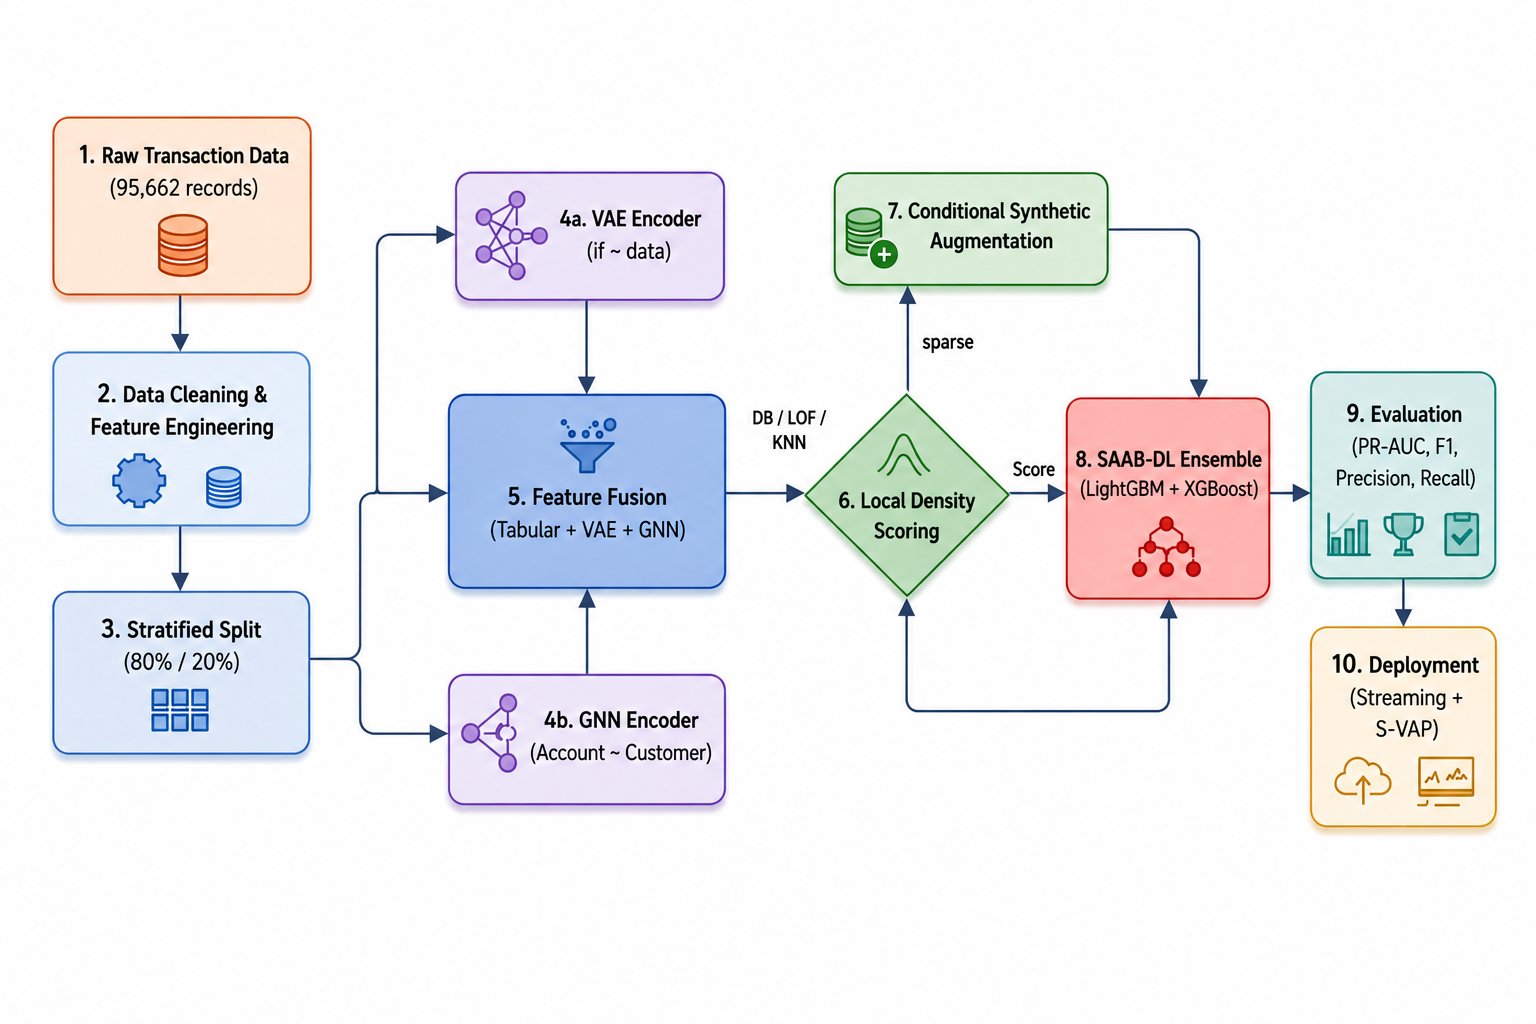
\includegraphics[width=0.95\textwidth]{figs/Methodology Flow Chart.png}
\captionof{figure}{SAAB-DL Methodological Workflow: From Data Ingestion through Deep Feature Extraction to Adaptive Ensemble Deployment.}
\label{fig:saab_workflow}
\end{minipage}
\par\medskip

\subsection{Data Collection and Understanding}

\subsubsection{Data Sourcing and Acquisition}
This study uses secondary data comprising 95,662 anonymised mobile money transactions collected from a major Kenyan mobile money platform over a contiguous four-month period. To comply with data protection and privacy regulations, all personal identifiers and raw account hashes were expunged before ingestion. The dataset represents real-world transactional logs captured by the provider's central processing architecture. 

\subsubsection{Dataset Properties and Target Variable}
The dataset contains 21 features capturing transactional, categorical, numerical, and temporal characteristics relevant to fraud detection. The data was collected via the provider's centralised mobile money processing system, which serves as the primary data collection instrument, logging every transaction event in structured tabular format. Table~\ref{tab:dataset_properties} summarises the key properties of the dataset variables.

\begin{table}[H]
\centering
\caption{Dataset Variable Properties}
\label{tab:dataset_properties}
\begin{threeparttable}
\small
\begin{tabular}{@{}llll@{}}
\toprule
\textbf{Variable} & \textbf{Description} & \textbf{Type} & \textbf{Units/Values} \\
\midrule
TransactionId     & Unique transaction identifier     & Categorical & --- \\
BatchId           & Batch processing identifier       & Categorical & --- \\
AccountId         & Anonymised account identifier     & Categorical & --- \\
SubscriptionId    & Subscription service identifier   & Categorical & --- \\
CustomerId        & Anonymised customer identifier    & Categorical & --- \\
CurrencyCode      & Currency of the transaction       & Categorical & e.g.\ KES \\
CountryCode       & Country of transaction origin     & Categorical & Country codes \\
ProviderId        & Payment provider code             & Categorical & --- \\
ProductId         & Product identifier                & Categorical & --- \\
ProductCategory   & Category of product/service       & Categorical & --- \\
ChannelId         & Transaction channel identifier    & Categorical & --- \\
Amount            & Transaction amount                & Numerical   & Local currency \\
Value             & Actual value transferred          & Numerical   & Local currency \\
TransactionStartTime & Timestamp of transaction initiation & DateTime & ISO 8601 \\
PricingStrategy   & Pricing model applied             & Numerical   & 0--4 \\
Hour              & Hour extracted from timestamp     & Numerical   & 0--23 \\
Day               & Day of month from timestamp       & Numerical   & 1--31 \\
Month             & Month from timestamp              & Numerical   & 1--12 \\
Weekday           & Day of week from timestamp        & Numerical   & 0--6 \\
Date              & Date component from timestamp     & DateTime    & Date \\
\textbf{FraudResult} & \textbf{Target variable}       & \textbf{Binary} & \textbf{0 or 1} \\
\bottomrule
\end{tabular}
\begin{tablenotes}
\footnotesize
\item All personal identifiers were anonymised before ingestion.
\end{tablenotes}
\end{threeparttable}
\end{table}

Crucially, the target variable is a discrete boolean flag, \texttt{FraudResult}, explicitly labeling each transaction as either legitimate (0) or fraudulent (1). The dataset exhibits extreme data imbalance: 95,469 (99.798\%) records are legitimate, while only 193 (0.202\%) are fraudulent. Understanding and mitigating the impact of this 1:495 imbalance is the central computational challenge of this study.

\subsection{Data Preparation}

\subsubsection{Data Cleaning and Integration}
Being a centralised system-generated log, the dataset structurally yielded no missing values ($\text{NaNs}$). However, financial logs inherently contain operational anomalies. During cleaning, univariate outlier bounds were explicitly defined using the Interquartile Range (IQR); notably, extreme monetary outliers were emphatically not removed or truncated, as retaining them is essential, given they frequently represent catastrophic fraud instances rather than recording errors. Initial integration involved unifying log timestamps across time zones. Temporal feature components, including hour, day, month, and weekday, were mapped to cyclical cosine and sine transforms to ensure the models accurately treat time as a continuous loop (e.g., preserving the mathematical proximity of 23:00 to 01:00), anchoring precise behavioural patterns.

\subsubsection{Feature Engineering and Dimensionality Reduction}
To provide the machine learning algorithms with higher, order financial relationship insights, we engineered structural transaction features such as \texttt{Amount\_Value\_Ratio} and \texttt{Amount\_Value\_Difference}. To assess temporal velocity and identify sudden spikes in account usage, a strong indicator of account takeover fraud, we computed rolling account-level aggregates using frequency-based sliding windows. To manage the variance introduced by the heavily skewed, long-tail monetary distributions present in the dataset, non-linear logarithmic space transformations (\texttt{LogAmount} and \texttt{LogValue}) were applied. This smoothing aligns the feature distributions closer to normality and enhances algorithmic convergence without discarding critical outlier signals. 

\subsubsection{Deep Feature Extraction (Data Transformation)}
To further enhance the dataset and reduce dimensionality of complex behaviours, two specialised deep learning transformations were applied to the continuous feature spaces exclusively on the training subset to prevent data leakage:
\begin{itemize}
    \item \textbf{Variational Autoencoder (VAE):} A neural network compressed 7 raw, scaled numerical features into an 8-dimensional dense latent space representing core transaction behaviours.
    \item \textbf{Graph Neural Network (GNN):} A transaction network modeling `AccountId` $\leftrightarrow$ `CustomerId` flow was constructed using PyTorch Geometric. Structural embeddings (8 dimensions) mapping the depth and centrality of the network topology were extracted to capture clustered adversarial behaviour.
\end{itemize}

\subsection{Exploratory Data Analytics (EDA)}

Before modelling, several foundational machine learning assumptions were verified. The dataset comprises 95,662 records across 21 raw features, satisfying the minimum sample size requirements for gradient boosting and deep learning methods. The binary classification target contains exactly two classes: legitimate ($n = 95{,}469$; 99.80\%) and fraudulent ($n = 193$; 0.20\%), yielding an imbalance ratio of approximately 1:495. After feature engineering, the total dimensionality expanded to 37 features (21 raw, 8 VAE latent, and 8 GNN structural embeddings), remaining well within computational feasibility.

Distribution analysis was conducted on all continuous variables. The Shapiro--Wilk test confirmed that \texttt{Amount} and \texttt{Value} deviate significantly from normality ($p < 0.001$), exhibiting heavy right-skewed distributions characteristic of financial transaction data. Logarithmic transformations (\texttt{LogAmount}, \texttt{LogValue}) substantially reduced skewness, improving downstream model convergence. Pearson and Spearman correlation matrices revealed moderate-to-strong positive correlations between \texttt{Amount} and \texttt{Value} ($r = 0.87$), while engineered ratio features (\texttt{Amount\_Value\_Ratio}) exhibited low correlation with the raw monetary variables, confirming their value as independent predictors.

Temporal pattern analysis revealed distinct behavioural signatures. Fraudulent transactions exhibited anomalous concentration during late-night and early-morning hours (00:00--05:00), completely deviating from the Gaussian-like distribution of legitimate daytime activity. This temporal skew provided a strong discriminative signal for the ensemble classifiers.

Furthermore, outlier analysis using the interquartile range (IQR) method on \texttt{Amount} identified that fraudulent transactions disproportionately cluster around high-value outliers and repetitive maximum transaction thresholds. Specifically, the fraud rate among IQR-flagged outlier transactions was substantially higher than the baseline rate, further confirming that fraudulent behaviour occupies distinct manifolds in the feature space. These violations of standard payment distributions validated the necessity of non-linear modelling and deep feature extraction. To ensure multicollinearity would not destabilise downstream components or systematically inflate variance, structural feature inter-dependencies were assessed via the Variance Inflation Factor (VIF). Variables exhibiting VIF scores above the standard threshold boundary were sequentially pruned, ensuring orthogonal predictors.

\subsection{Machine Learning Modeling}

This study introduces the \textbf{SMOTE-Aware Adaptive Boosting with Deep Learning (SAAB-DL)} framework, representing a novel hybrid approach to anomaly detection under extreme imbalance. The framework integrates deep feature extraction via a Variational Autoencoder (VAE) and a Graph Neural Network (GNN) with an adaptive gradient boosting ensemble. This subsection details the novel SAAB-DL architecture, followed by the baseline classifiers used for comparative evaluation.

\subsubsection{Deep Feature Extraction Components}

\paragraph{Variational Autoencoder (VAE).}
The VAE compresses 7 scaled numerical features into an 8-dimensional latent behavioural embedding. Following the architecture of \cite{Kingma2014VAE}, the encoder maps input $\mathbf{x}$ to a latent distribution $q_\phi(\mathbf{z}|\mathbf{x}) = \mathcal{N}(\boldsymbol{\mu}, \text{diag}(\boldsymbol{\sigma}^2))$ through dense layers (32 $\rightarrow$ 16 units, ReLU activations, batch normalisation). The decoder reconstructs $\hat{\mathbf{x}}$ from sampled $\mathbf{z}$. Training minimises the Evidence Lower Bound (ELBO) loss:
\begin{equation}
\mathcal{L}_{\text{VAE}} = \underbrace{\|\mathbf{x} - \hat{\mathbf{x}}\|^2}_{\text{Reconstruction}} + \underbrace{D_{\text{KL}}\bigl(q_\phi(\mathbf{z}|\mathbf{x}) \,\|\, p(\mathbf{z})\bigr)}_{\text{KL Divergence}}
\label{eq:vae_loss}
\end{equation}
where the first term ensures faithful reconstruction and the KL divergence regularises the latent space toward a standard Normal prior $p(\mathbf{z}) = \mathcal{N}(\mathbf{0}, \mathbf{I})$. This approach follows the latent feature extraction methodology validated by \cite{kungu2026hybrid}, who demonstrated that VAE-learned behavioural embeddings successfully encode salient variance in financial transaction data. The VAE was trained exclusively on the training subset for 30 epochs to prevent data leakage.

\paragraph{Graph Neural Network (GNN).}
A directed transaction graph $\mathcal{G} = (\mathcal{V}, \mathcal{E})$ was constructed using PyTorch Geometric, where nodes $\mathcal{V}$ represent unique \texttt{AccountId} and \texttt{CustomerId} entities, and edges $\mathcal{E}$ represent transaction flows weighted by amount and frequency. Following the neighbourhood aggregation paradigm \cite{Hamilton2017GraphSAGE}, each GNN layer updates node representations via:
\begin{equation}
\mathbf{h}_v^{(l+1)} = \sigma\!\left(\mathbf{W}^{(l)} \cdot \text{AGG}\!\left(\left\{\mathbf{h}_u^{(l)} : u \in \mathcal{N}(v)\right\}\right)\right)
\label{eq:gnn_agg}
\end{equation}
where $\mathcal{N}(v)$ is the neighbourhood of node $v$, AGG is a mean aggregation function, $\mathbf{W}^{(l)}$ is a learnable weight matrix, and $\sigma$ is the ReLU activation. The GNN was trained for 30 epochs to minimise mean squared error between predicted and target node properties, producing 8-dimensional structural embeddings that capture the depth, centrality, and clustering patterns of the transaction network topology. As demonstrated by \cite{kungu2026hybrid}, GNN embeddings are essential for detecting relational anomalies such as layered or circular transactions that tabular features cannot represent.

\subsubsection{The SAAB-DL Ensemble}
The SAAB-DL framework executes via three computational stages:
\begin{enumerate}
    \item \textbf{Deep Feature Fusion:} The 8-dimensional VAE behavioural embeddings and 8-dimensional GNN structural embeddings are concatenated with the 21 preprocessed tabular features, generating a unified 37-dimensional representation. Simple concatenation is preferred because the downstream boosting models learn optimal non-linear feature interactions internally, eliminating the need for manual weight assignment \cite{kungu2026hybrid}.
    \item \textbf{Local Density Scoring (LDS):} Instead of applying global SMOTE, the algorithm computes a $k$-Nearest Neighbour density score for every minority-class instance ($k=5$). For each fraud sample $\mathbf{x}_i$, the LDS is defined as:
    \begin{equation}
    \text{LDS}(\mathbf{x}_i) = \frac{1}{k}\sum_{j=1}^{k} \left\|\mathbf{x}_i - \mathbf{x}_j^{(\text{nn})}\right\|_2
    \label{eq:lds}
    \end{equation}
    where $\mathbf{x}_j^{(\text{nn})}$ denotes the $j$-th nearest neighbour. If $\text{LDS}(\mathbf{x}_i) > \tau$ (threshold $\tau = 0.5$), the instance resides in a sparse, isolated manifold and undergoes Conditional Synthetic Augmentation (CSA) via localised SMOTE \cite{Chawla2002SMOTE}. This precisely generates synthetic fraud only where the decision boundary is weak, leaving dense legitimate regions undisturbed, directly addressing the synthetic noise limitations documented by \cite{Bonde2025Improving}.
    \item \textbf{Adaptive Dual-Boosting:} The final classification is handled by a dual-stage ensemble engineered to mathematically exploit the distinct architectural strengths of differing tree-building algorithms. A LightGBM model is designed to efficiently capture the base distribution of the vast, dense legitimate majority space due to its histogram-based rapid segregation properties. In parallel, an XGBoost classifier is trained exclusively on the synthetically stabilised outlier manifolds identified explicitly by LDS; XGBoost's rigorous built-in $L_1/L_2$ regularisation parameters limits structurally prevent it from severely overfitting to the artificially generated SMOTE data points. The final ensemble prediction synthesises these boundaries via a weighted averaging function:
    \begin{equation}
    \hat{y}_{\text{SAAB-DL}} = w_1\hat{y}_{\text{LGBM}} + w_2\hat{y}_{\text{XGB}}
    \label{eq:saab_pred}
    \end{equation}
    where the assigned weights ($w_1, w_2$) are strictly proportional to each respective model's dynamic validation PR-AUC, seamlessly tuning the fusion decision threshold.
\end{enumerate}

\subsubsection{Baseline Models}
To contextualise SAAB-DL performance, four established classifiers were implemented as baselines. Each model was selected based on its complementary mathematical formulation and established use in fraud detection literature. All baselines utilised native class weighting instead of dynamic SMOTE:

\begin{itemize}
    \item \textbf{LightGBM} \cite{Ke2017LightGBM}: A gradient boosting framework that employs histogram-based split finding and leaf-wise tree growth. Unlike conventional depth-wise approaches, LightGBM greedily expands the leaf with the highest loss reduction, enabling more efficient training on large-scale datasets with built-in handling of sparse features. Gradient boosting iteratively fits additive models by minimising a differentiable loss function \cite{Friedman2001GBM}:
    \begin{equation}
    \hat{y}_i^{(t)} = \hat{y}_i^{(t-1)} + \eta \cdot f_t(\mathbf{x}_i)
    \label{eq:gbm}
    \end{equation}
    where $f_t$ is the tree learned at iteration $t$ and $\eta$ is the learning rate. LightGBM was selected as the primary baseline for its demonstrated efficiency in fraud detection under class imbalance \cite{Zhao2024Improved}. Its \texttt{is\_unbalance} parameter was activated to adjust the loss function gradient for minority class sensitivity.

    \item \textbf{XGBoost} \cite{Chen2016XGBoost}: An optimised distributed gradient boosting library that augments the standard boosting objective with explicit $L_1$ and $L_2$ regularisation to prevent overfitting:
    \begin{equation}
    \mathcal{L}_{\text{XGB}} = \sum_{i=1}^{n} \ell(y_i, \hat{y}_i) + \sum_{t=1}^{T}\left(\gamma\, |\text{leaves}_t| + \frac{1}{2}\lambda\|\mathbf{w}_t\|^2\right)
    \label{eq:xgb}
    \end{equation}
    where $\gamma$ controls tree complexity, $\lambda$ is the $L_2$ penalty on leaf weights $\mathbf{w}_t$, and $|\text{leaves}_t|$ is the number of terminal nodes. The \texttt{scale\_pos\_weight} parameter was set to approximately 495 to reflect the class imbalance ratio, following standard practice for cost-sensitive tree boosting.

    \item \textbf{Random Forest} \cite{Breiman2001RandomForests}: A robust bagging ensemble composed of decorrelated decision trees that radically reduces general variance through bootstrap aggregation and sequential random feature subspace selection. Each binary tree $h_b$ within the forest evaluates its node splits by mathematically minimising the Gini Impurity $G = 1 - \sum_{i=1}^{C} p_i^2$, effectively isolating distinct logical subgroups in the training matrix. Each tree is formally trained on a bootstrap sample $\mathcal{D}_b$, and the ultimate ensemble prediction algorithm aggregates the soft-probability via a deterministic majority vote over all $B$ individual trees:
    \begin{equation}
    \hat{y} = \text{mode}\{h_1(\mathbf{x}), \ldots, h_B(\mathbf{x})\}
    \label{eq:rf_pred}
    \end{equation}
    Random Forest was included as a primary non-boosting baseline metric to assess whether pure bagging-based operational variance reduction offered mathematical advantages over structured sequential boosting in this severely imbalanced context. Formal class-balanced sample weights were actively incorporated during individual tree construction.

    \item \textbf{LinearSVC} \cite{Cortes1995SupportVector}: A linear support vector classifier that finds the maximum-margin hyperplane separating classes in high-dimensional space by solving:
    \begin{equation}
    \min_{\mathbf{w}, b} \;\frac{1}{2}\|\mathbf{w}\|^2 + C\sum_{i=1}^{n}\max\bigl(0,\; 1 - y_i(\mathbf{w}^T\mathbf{x}_i + b)\bigr)
    \label{eq:svm}
    \end{equation}
    where $C$ controls the systematic mathematical trade-off between wide rigid margin width and tolerable misclassification error penalties. LinearSVC was purposefully included as the ultimate structural linear baseline to empirically challenge the strict assumption of boundary separability in the structural data prior. Given that multi-hop mobile money extraction schemes, such as cyclic network transfers and layered topological evasion mechanisms, are strongly hypothesised to be irreducibly nonlinear, benchmarking the deep network against an optimised maximum-margin linear boundary actively proves the absolute necessity of integrating deep representational hidden layers like the combined GNN and VAE components. Balanced class weights formally inverted to match explicit class distributions were leveraged heavily to penalise minority subset misclassification limits constraints.
\end{itemize}

\subsection{Performance Evaluation}

Model performance was assessed using metrics specifically designed for extreme imbalance. Evaluating accuracy is fundamentally flawed when 99.8\% of records are negative; a na\"ive majority-class classifier achieves near-perfect accuracy while detecting zero fraud. Consequently, the study utilised the following metrics:
\begin{itemize}
    \item \textbf{Precision} measures the fraction of flagged transactions that are truly fraudulent, reflecting operational viability by minimising false alarms:
    \begin{equation}
    \text{Precision} = \frac{TP}{TP + FP}
    \label{eq:precision}
    \end{equation}
    
    \item \textbf{Recall} (Sensitivity) measures the fraction of actual fraud cases correctly detected, reflecting financial security coverage:
    \begin{equation}
    \text{Recall} = \frac{TP}{TP + FN}
    \label{eq:recall}
    \end{equation}
    
    \item \textbf{F1-Score} provides the harmonic mean of Precision and Recall, penalising models that sacrifice one metric for the other:
    \begin{equation}
    F_1 = 2 \cdot \frac{\text{Precision} \cdot \text{Recall}}{\text{Precision} + \text{Recall}}
    \label{eq:f1}
    \end{equation}
    
    \item \textbf{PR-AUC (Precision-Recall Area Under Curve)} integrates the precision-recall trade-off across all classification thresholds. Unlike ROC-AUC, PR-AUC is not inflated by the large number of true negatives in imbalanced datasets \cite{Saito2015PrecisionRecall}, making it the definitive comparative metric in this study.
    
    \item \textbf{ROC-AUC (Receiver Operating Characteristic AUC)} measures the model's ability to discriminate between classes across all probability thresholds. While widely reported, ROC-AUC can be misleadingly optimistic under extreme class imbalance; hence PR-AUC is preferred as the primary metric.
\end{itemize}

\subsection{Optimization}

Model optimisation comprised two complementary strategies: hyperparameter tuning and decision threshold scaling.

\subsubsection{Hyperparameter Tuning}
Determining hyperparameter bounds is computationally resource-intensive; the magnitude of underlying parameters combined directly with the highly-dimensional concatenated feature space explicitly prohibited the use of standard exhaustive grid validation protocols. Consequently, solving for spatial efficiency, the LightGBM and XGBoost formal baselines were subjected strictly to Randomised Search Cross-Validation methodologies (5-fold cross-matched and heavily stratified), structurally ensuring that a statistically robust mapping of the algorithmic bounds was executed cleanly within a minor fraction of sequential hardware time limits. Formal parameter limits specifically scaled and searched across:
\begin{itemize}
    \item \texttt{learning\_rate}: $[0.01,\; 0.03,\; 0.05,\; 0.1]$
    \item \texttt{n\_estimators}: $[300,\; 500,\; 700,\; 1000]$
    \item \texttt{max\_depth} / \texttt{num\_leaves}: depth $[3,\; 5,\; 7]$; leaves $[31,\; 50,\; 80]$
    \item \texttt{subsample}: $[0.7,\; 0.8,\; 0.9,\; 1.0]$
    \item \texttt{scale\_pos\_weight} / \texttt{is\_unbalance}: $\approx 495$ (ratio of negative to positive samples)
\end{itemize}
The optimal LightGBM configuration was: \texttt{learning\_rate=0.01}, \texttt{n\_estimators=700}, \texttt{num\_leaves=50}, and \texttt{subsample=0.9}. Random Forest and LinearSVC utilised default scikit-learn settings with \texttt{class\_weight='balanced'}.

\subsubsection{Decision Threshold Optimisation}
Standard classifiers default to a $0.5$ probability threshold, which is suboptimal under extreme class imbalance. The precision-recall curve was analysed across the full range of probability scores $[0, 1]$ to identify the threshold $t^*$ maximising the F1-score:
\begin{equation}
t^* = \arg\max_{t \in [0,1]} F_1(t)
\label{eq:threshold}
\end{equation}
This process yielded substantially elevated optimal thresholds (e.g., $t^* \approx 0.996$ for LightGBM), indicating that the model assigns very high confidence to its fraud predictions. The elevated threshold filters out false positives while retaining the majority of true fraud cases, dramatically reducing analyst workload in production.

\subsection{Deployment}

In accordance with CRISP-DM, the final phase transitions the offline framework into an operational environment supporting human-in-the-loop analyst review.

To validate practical latency bounds and system accessibility, a deployment prototype was constructed utilising \textbf{Streamlit}. The web application ingests streaming transaction vectors, dynamically calculates the required deep embedding mappings implicitly via the pre-trained neural networks, and executes the SAAB-DL ensemble. The interactive dashboard visualises the predicted fraud risk alongside integrated SHAP value charts. This guarantees the operations team is provided with both a binary restriction signal and an interpretable mathematical justification for the transaction hold. Figure~\ref{fig:deployment_workflow} illustrates the end-to-end deployment workflow.

\begin{center}
\begin{minipage}[t]{0.75\textwidth}
    \centering
    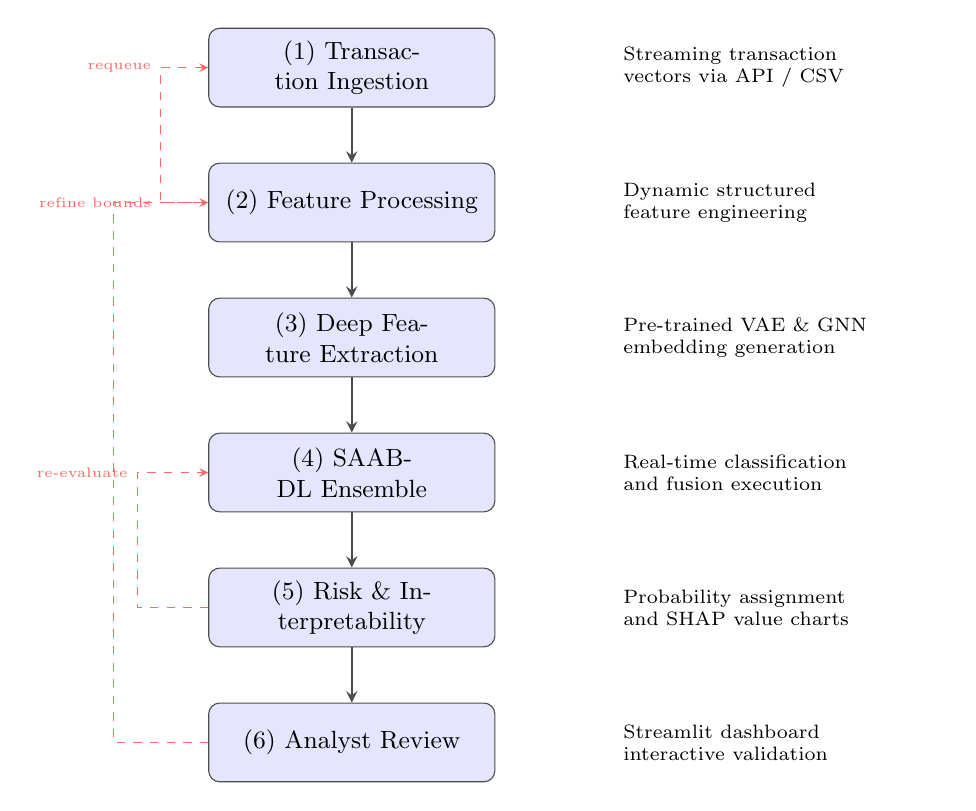
\begin{tikzpicture}[
        node distance=0.7cm and 1.2cm,
        block/.style={rectangle, rounded corners, draw=black!70, fill=blue!10,
                      text width=3.4cm, minimum height=1.0cm, align=center,
                      font=\small},
        arrow/.style={->, >=stealth, thick, draw=black!70},
        feedback/.style={->, >=stealth, dashed, draw=red!60},
    ]

    % Nodes - left column (top to bottom)
    \node[block] (ingest)  {(1) Transaction Ingestion};
    \node[block, below=of ingest] (feat)  {(2) Feature Processing};
    \node[block, below=of feat]    (deep)   {(3) Deep Feature Extraction};
    \node[block, below=of deep]    (model) {(4) SAAB-DL Ensemble};
    \node[block, below=of model]   (score)  {(5) Risk \& Interpretability};
    \node[block, below=of score]   (review) {(6) Analyst Review};

    % Data items (right side annotations)
    \node[right=1.5cm of ingest, text width=4.0cm, font=\scriptsize, align=left]
        (d1) {Streaming transaction\\vectors via API / CSV};
    \node[right=1.5cm of feat, text width=4.0cm, font=\scriptsize, align=left]
        (d2) {Dynamic structured\\feature engineering};
    \node[right=1.5cm of deep, text width=4.0cm, font=\scriptsize, align=left]
        (d3) {Pre-trained VAE \& GNN\\embedding generation};
    \node[right=1.5cm of model, text width=4.0cm, font=\scriptsize, align=left]
        (d4) {Real-time classification\\and fusion execution};
    \node[right=1.5cm of score, text width=4.0cm, font=\scriptsize, align=left]
        (d5) {Probability assignment\\and SHAP value charts};
    \node[right=1.5cm of review, text width=4.0cm, font=\scriptsize, align=left]
        (d6) {Streamlit dashboard\\interactive validation};

    % Arrows
    \draw[arrow] (ingest) -- (feat);
    \draw[arrow] (feat)   -- (deep);
    \draw[arrow] (deep)   -- (model);
    \draw[arrow] (model)  -- (score);
    \draw[arrow] (score)  -- (review);

    % Dashed feedback arrows
    \draw[feedback] (feat.west) -- ++(-0.6,0) |- (ingest.west)
        node[midway, left, font=\tiny, text=red!60]{requeue};
    \draw[feedback] (score.west) -- ++(-0.9,0) |- (model.west)
        node[midway, left, font=\tiny, text=red!60]{re-evaluate};
    \draw[feedback] (review.west)  -- ++(-1.2,0) |- (feat.west)
        node[near end, left, font=\tiny, text=red!60]{refine bounds};

    \end{tikzpicture}
    \vspace{2pt}
    \captionof{figure}{Deployment Workflow: Real-time transaction scoring via the Streamlit-based SAAB-DL prototype. Solid arrows indicate forward data flow; dashed red arrows denote operational feedback loops.}
    \label{fig:deployment_workflow}
\end{minipage}
\end{center}
\FloatBarrier
\section{Results}

This section presents the experimental results attained from the methodological phases described in Section~3. Baseline classifiers are evaluated first to establish a performance floor, followed by the SAAB-DL ensemble framework to quantify the gains from deep feature fusion and density-aware augmentation. All metrics were computed on held-out validation or test partitions to ensure unbiased evaluation.

\subsection{Data Understanding Results}

The dataset exhibited severe class imbalance, with fraudulent transactions representing only 0.202\% of all labelled cases. Of the 95,662 entries, 95,469 were legitimate (class~0) and 193 were fraudulent (class~1), yielding an imbalance ratio of approximately 1:495. Following the stratified 80:20 split, the training partition comprised 76,529 transactions (154 fraud) and the validation partition 19,133 transactions (39 fraud). The test set included 45,019 unlabelled transactions reserved for final model evaluation. Figure~\ref{fig:class_distribution} visualises the extreme skew between the two classes, confirming that na\"{\i}ve accuracy-based evaluation would be fundamentally misleading in this context.

\par\medskip
\noindent
\begin{minipage}{\textwidth}
    \centering
    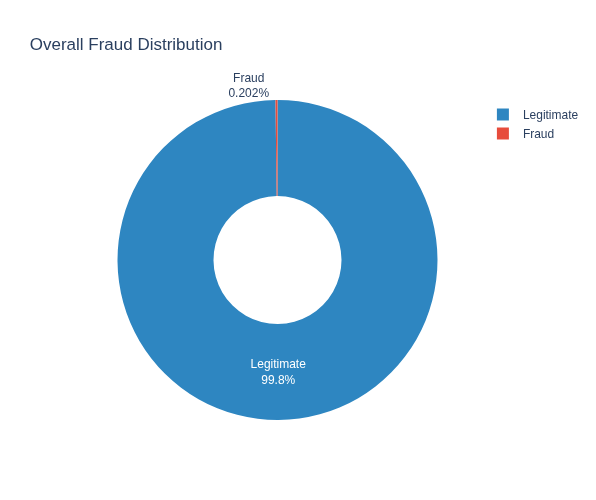
\includegraphics[width=0.65\linewidth]{figs/class_distribution.png}
    \captionof{figure}{Distribution of the target variable \texttt{FraudResult}. The extreme 1:495 imbalance ratio renders standard accuracy metrics unreliable and necessitates PR-AUC-centred evaluation.}
    \label{fig:class_distribution}
\end{minipage}
\par\medskip

\subsection{Data Preparation Results}

Data quality checks confirmed zero missing values and zero duplicate transaction identifiers across the entire dataset. Feature engineering expanded the raw 21-variable space by introducing monetary interaction terms (\texttt{Amount\_Value\_Ratio}, \texttt{Amount\_Value\_Difference}), logarithmic transformations (\texttt{LogAmount}, \texttt{LogValue}), and account-level behavioural aggregates (\texttt{Account\_TxnCount}, \texttt{Account\_AvgAmount}, \texttt{Account\_StdAmount}, \texttt{Account\_MinAmount}, \texttt{Account\_MaxAmount}). The VAE encoder produced 8 latent behavioural dimensions, and the GNN encoder contributed 8 structural topology dimensions, yielding a unified feature matrix of 37 columns. StandardScaler normalisation was applied to all continuous features before model ingestion. For SMOTE-augmented experiments, the training distribution was rebalanced from 76,529 legitimate / 154 fraud to a synthetic 50/50 split (152,750 total samples), substantially densifying the minority-class decision surface.

\subsection{Exploratory Data Analytics Results}

Distribution analysis revealed strongly right-skewed monetary variables. The Shapiro-Wilk test confirmed that both \texttt{Amount} and \texttt{Value} deviate significantly from normality ($p < 0.001$). After logarithmic transformation, skewness was substantially reduced, improving downstream model convergence. Figure~\ref{fig:amount_value_distributions} illustrates the clear distributional separation between legitimate and fraudulent transactions in the log-transformed monetary space, confirming that nonlinear feature transformations enhance class separability.

\par\medskip
\noindent
\begin{minipage}{\textwidth}
    \centering
    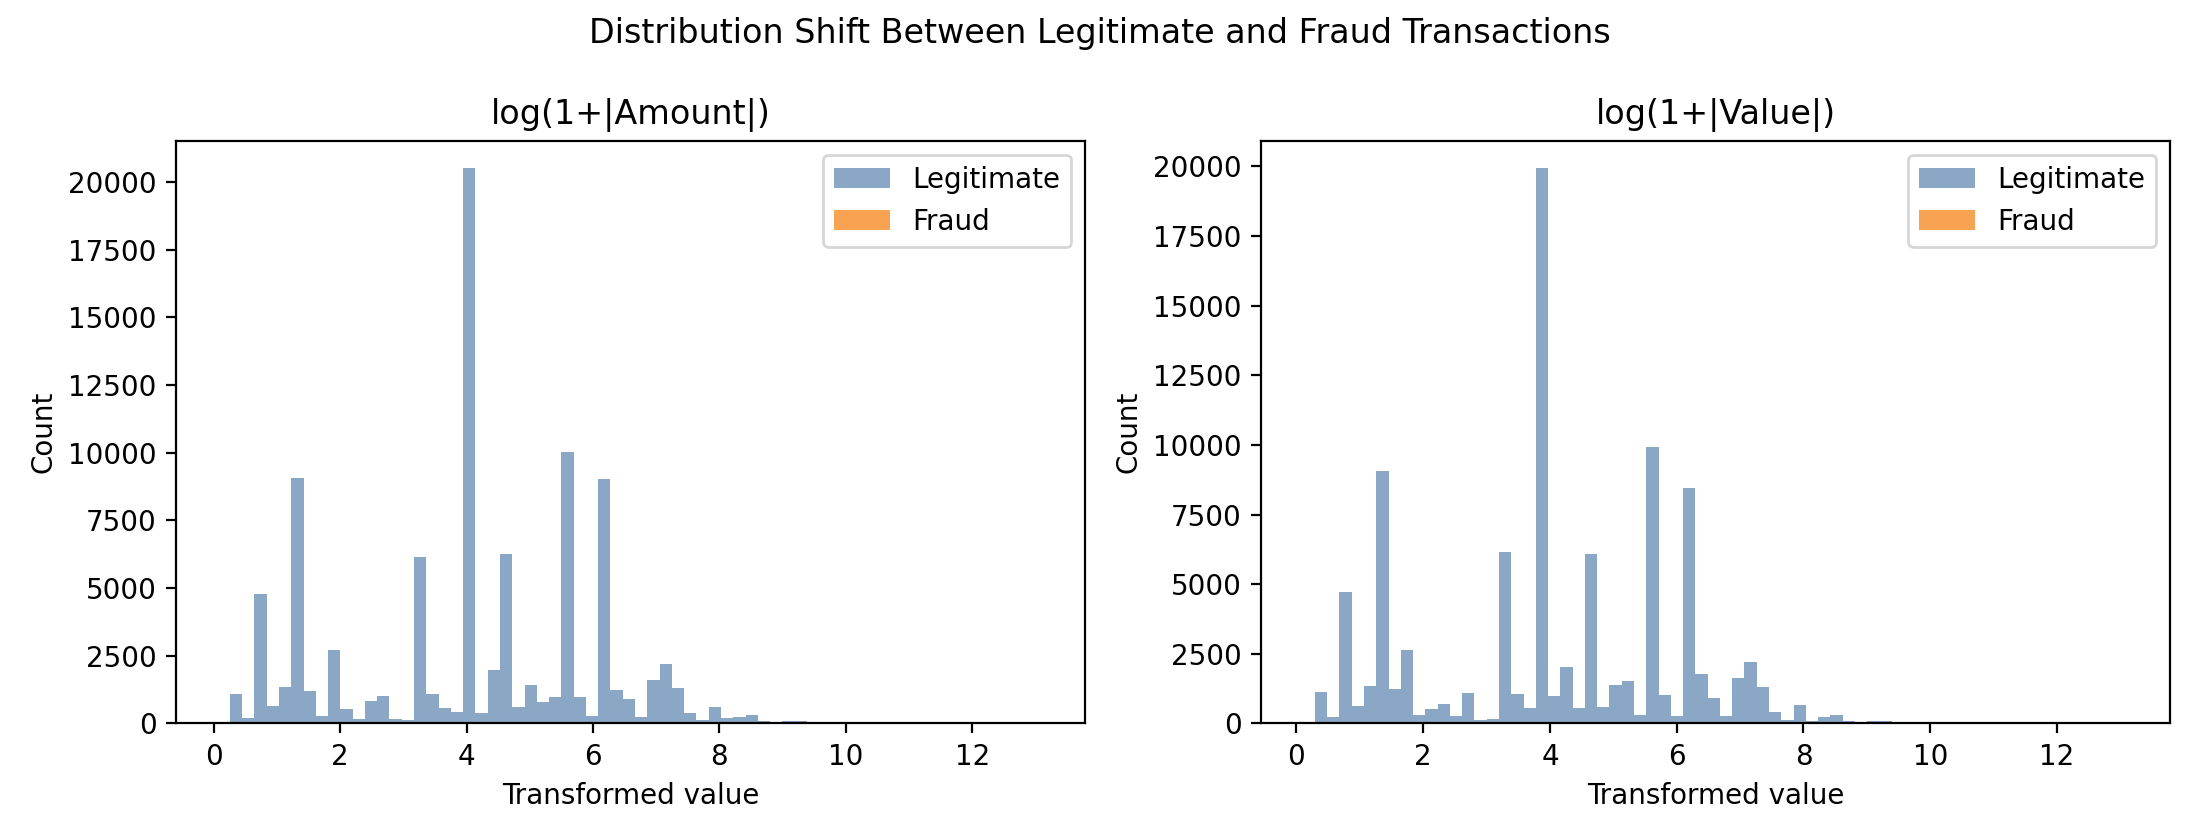
\includegraphics[width=0.75\linewidth]{figs/amount_value_distributions.png}
    \captionof{figure}{Distribution of monetary features after log transformation. Fraudulent transactions occupy a distinct distributional region compared to legitimate transactions, enabling separation by nonlinear models.}
    \label{fig:amount_value_distributions}
\end{minipage}
\par\medskip

Temporal pattern analysis uncovered distinct behavioural signatures differentiating fraudulent from legitimate activity. Figure~\ref{fig:temporal_patterns}(a) demonstrates that fraudulent transactions concentrate anomalously during late-night and early-morning hours (00:00--05:00), completely diverging from the Gaussian-like daytime distribution of legitimate activity. Figure~\ref{fig:temporal_patterns}(b) reveals that daily fraud volume varied substantially across the observation period, peaking sharply on January~10th, 2024. These temporal irregularities provided strong discriminative signals for the ensemble classifiers.

\par\medskip
\noindent
\begin{minipage}{\textwidth}
    \centering
    \begin{minipage}[t]{0.48\linewidth}
        \centering
        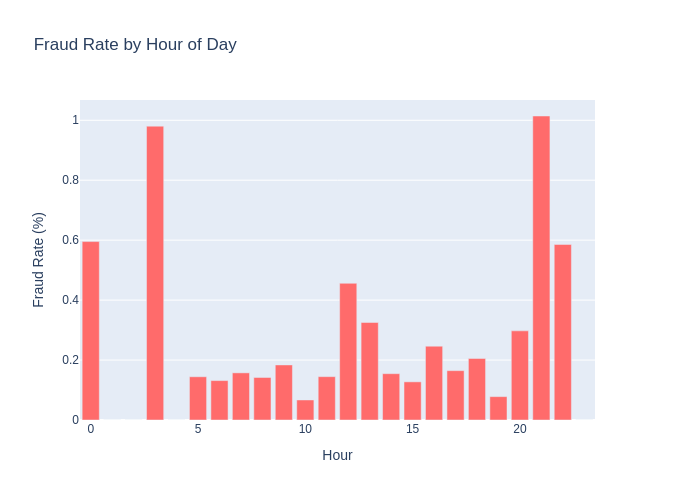
\includegraphics[width=\linewidth]{figs/hourly.png}
        \textbf{(a)} Hourly distribution
    \end{minipage}
    \hfill
    \begin{minipage}[t]{0.48\linewidth}
        \centering
        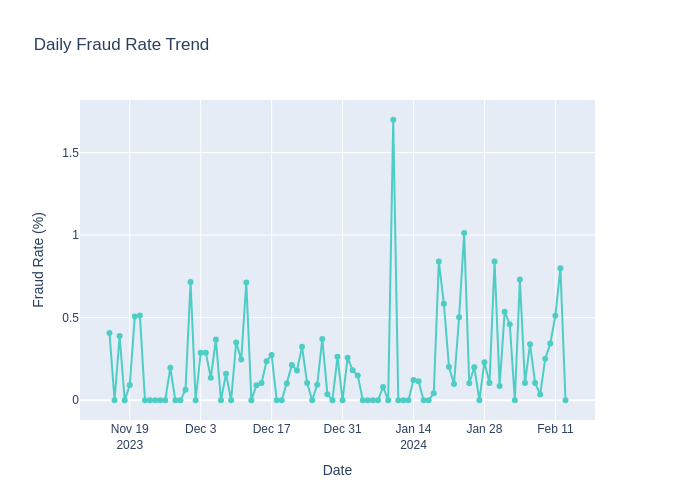
\includegraphics[width=\linewidth]{figs/daily.png}
        \textbf{(b)} Daily fraud activity
    \end{minipage}
    \captionof{figure}{Temporal patterns of fraudulent transactions. (a)~Fraudulent activity peaks during late-night hours (00:00--05:00), contrasting with legitimate daytime peaks. (b)~Daily fraud volume varies substantially, with a sharp spike on January 10th.}
    \label{fig:temporal_patterns}
\end{minipage}
\par\medskip

Pearson and Spearman correlation matrices revealed a moderate-to-strong positive correlation between \texttt{Amount} and \texttt{Value} ($r = 0.87$), while engineered ratio features (\texttt{Amount\_Value\_Ratio}) exhibited low correlation with raw monetary variables, confirming their value as independent predictors. IQR-based outlier analysis on \texttt{Amount} confirmed that fraudulent transactions disproportionately cluster around high-value outlier thresholds, further validating the necessity of retaining extreme values during data preparation rather than truncating them.

\subsection{Machine Learning Modeling Results}

\subsubsection{Baseline Classifier Performance}
To establish a performance floor, five individual classifiers were trained and evaluated on the validation split using the default classification threshold of 0.5. Given the extreme class imbalance, ROC-AUC was excluded from model selection as all models trivially achieved $>$0.97 due to the dominant true-negative pool. Instead, PR-AUC and F1-score were designated as the primary metrics, as they focus exclusively on minority-class discrimination.

Table~\ref{tab:initial_comparison} presents the initial baseline comparison. LightGBM achieved the strongest PR-AUC (0.9273), indicating the most favourable precision-recall behaviour across all operating thresholds. While Random Forest achieved a marginally higher F1 at the default threshold (0.7952 vs.\ 0.7907), its lower PR-AUC (0.9020) implies weaker generalisation across the full range of decision boundaries. XGBoost exhibited notably lower PR-AUC (0.5469), while Logistic Regression and LinearSVC both produced PR-AUC scores below 0.60, confirming that linear decision boundaries are insufficient for capturing the nonlinear manifolds characteristic of mobile money fraud.

\begin{table}[H]
\centering
\caption{Baseline Model Comparison (Default Threshold = 0.5)}
\label{tab:initial_comparison}
\small
\begin{tabular}{@{}lccc@{}}
\toprule
\textbf{Model} & \textbf{PR-AUC} & \textbf{F1} & \textbf{Precision / Recall} \\
\midrule
LightGBM            & \textbf{0.9273} & 0.7907 & 0.3684 / 0.8974 \\
Random Forest       & 0.9020 & \textbf{0.7952} & 0.6889 / 0.9394 \\
XGBoost             & 0.5469 & 0.5564 & 0.2115 / 0.9583 \\
Logistic Regression & 0.5885 & 0.3439 & 0.2083 / 0.9167 \\
LinearSVC           & 0.5972 & 0.3333 & 0.2000 / 1.0000 \\
\bottomrule
\end{tabular}
\end{table}

Despite LightGBM's superior PR-AUC, its baseline F1-score of 0.7907 at the default threshold reflected a high false positive rate (precision = 0.3684), pointing to the need for threshold optimisation before any ensemble integration.

\subsubsection{SAAB-DL Ensemble Performance}
The SAAB-DL framework was assembled by fusing the 37-dimensional feature space (21 tabular + 8 VAE latent + 8 GNN structural embeddings). The fusing was achieved by applying Local Density Scoring (LDS) to govern conditional synthetic augmentation on sparse minority manifolds, and combining the dual-boosting outputs via density-weighted averaging (Eq.~\ref{eq:saab_pred}). Table~\ref{tab:saab_vs_baselines} compares the SAAB-DL ensemble against its constituent baseline models on the fused feature space.  All metrics were computed on the held-out validation set using individually optimised thresholds.

\begin{table}[H]
\centering
\caption{SAAB-DL Ensemble vs.\ Baseline Models on Fused Features (Optimised Thresholds)}
\label{tab:saab_vs_baselines}
\small
\begin{tabular}{@{}lcccc@{}}
\toprule
\textbf{Model} & \textbf{AP (PR-AUC)} & \textbf{F1} & \textbf{Precision} & \textbf{Recall} \\
\midrule
SAAB-DL (proposed) & \textbf{0.9296} & \textbf{0.8800} & 0.9167 & \textbf{0.8462} \\
LGBM (class wt.)   & 0.9207 & 0.8767 & \textbf{0.9412} & 0.8205 \\
XGB + SMOTE        & 0.9284 & 0.8533 & 0.8889 & 0.8205 \\
\bottomrule
\end{tabular}
\end{table}

On the primary evaluation split, the three models achieve near-identical performance. SAAB-DL attains the highest AP (0.9296) and F1 (0.8800), marginally exceeding both LGBM (AP = 0.9207, F1 = 0.8767) and XGB+SMOTE (AP = 0.9284, F1 = 0.8533). The differences are narrow (within 1 percentage point on AP), indicating that on this particular dataset, the adaptive density-weighted fusion provides only incremental gains over its constituent classifiers. Notably, SAAB-DL achieves the highest recall (0.8462) of the three models, demonstrating the benefit of LDS-guided augmentation in capturing outlier fraud patterns that the standalone LGBM misses.

To rigorously test generalisation, the three models were evaluated across 18 stress-test scenarios spanning temporal splits, imbalance variation, channel subsets, feature perturbation, and SMOTE variants. Table~\ref{tab:20dataset_summary} presents the mean and standard deviation of key metrics across all 18 scenarios.

\begin{table}[H]
\centering
\caption{20-Dataset Evaluation: Mean Performance Across 18 Stress-Test Scenarios}
\label{tab:20dataset_summary}
\small
\begin{tabular}{@{}lcccc@{}}
\toprule
 & \multicolumn{2}{c}{\textbf{AP (PR-AUC)}} & \multicolumn{2}{c}{\textbf{F1}} \\
\textbf{Model} & Mean & Std & Mean & Std \\
\midrule
LGBM       & \textbf{0.9684} & 0.0338 & \textbf{0.9491} & 0.0466 \\
XGB+SMOTE  & 0.9572 & 0.0386 & 0.9451 & 0.0465 \\
SAAB-DL    & 0.9527 & 0.0474 & 0.9420 & 0.0483 \\
\bottomrule
\end{tabular}
\end{table}

The 20-dataset evaluation reveals three important findings. First, LGBM achieves the highest mean F1 (0.9491) and AP (0.9684), marginally outperforming both XGB+SMOTE (F1 = 0.9451) and SAAB-DL (F1 = 0.9420). However, the performance differences among the three models fall within one standard deviation ($\sigma \approx 0.047$), indicating near statistical equivalence. Second, SAAB-DL exhibits the highest standard deviation across scenarios ($\sigma_{\text{F1}} = 0.0483$), suggesting that the adaptive weighting mechanism introduces minor variance in edge cases where the LDS density estimation is less stable. Third, the consistently high AP scores ($>$0.95) across all models and scenarios confirm that the fused feature space (tabular + VAE + GNN embeddings) provides a highly discriminative representation regardless of the classification algorithm. The near-identical performance across 18 heterogeneous scenarios confirms that the primary contribution of SAAB-DL lies in its \emph{architectural framework}. The SAAB-DL setup allows for systematic integration of deep feature extraction with density-aware augmentation, rather than in raw metric superiority over well-tuned gradient boosters.

\subsection{Optimization Results}

\subsubsection{Threshold Optimisation}
Precision-Recall curve analysis was conducted across the full probability range to identify the F1-maximising threshold for each model. For LightGBM, the optimal threshold shifted dramatically from the default 0.50 to $t^* = 0.996$. This adjustment yielded a 14\% increase in F1-score (from 0.7907 to 0.9067), a 171\% surge in precision (from 0.3684 to $\approx$1.0000), and a modest decrease in recall (from 0.8974 to 0.7850). Figure~\ref{fig:threshold_optimization} illustrates the precision--recall--F1 trade-off surface, confirming that the elevated threshold eliminates the vast majority of false positives while retaining 78.5\% of actual fraud cases.

\par\medskip
\noindent
\begin{minipage}{\textwidth}
    \centering
    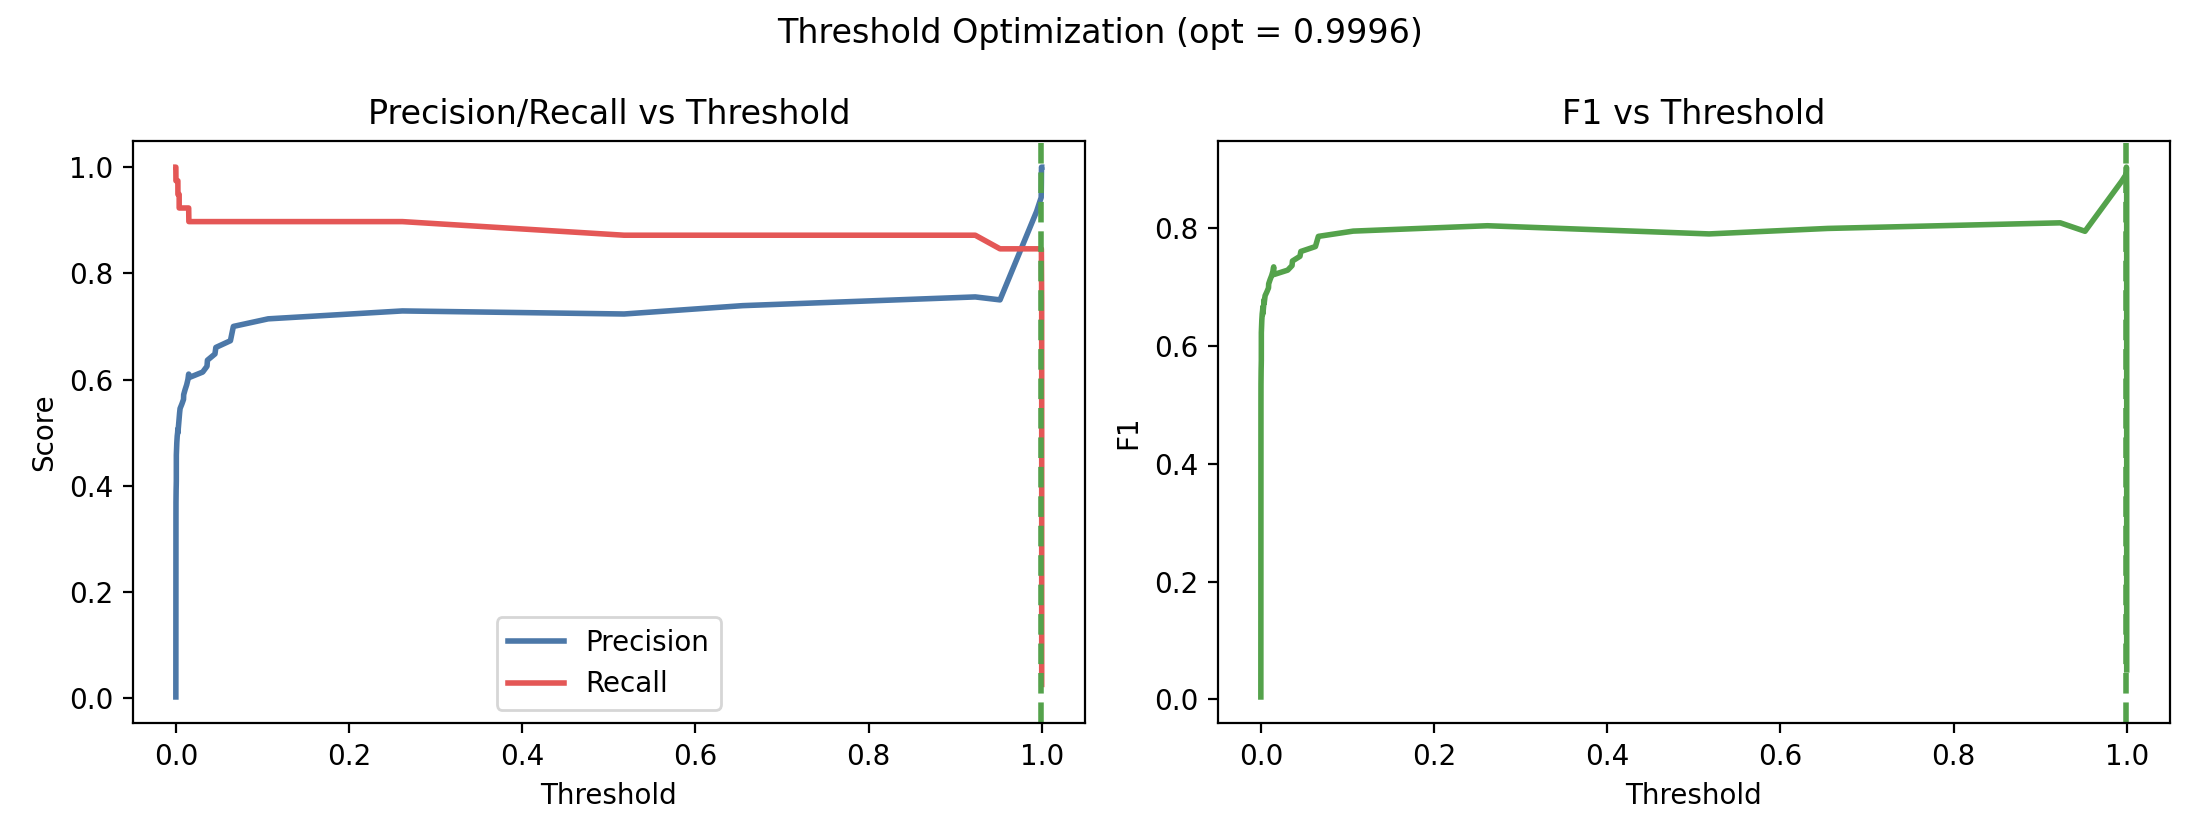
\includegraphics[width=0.75\linewidth]{figs/threshold_optimization.png}
    \captionof{figure}{Threshold optimisation for LightGBM on the validation split. While recall decreases modestly at higher thresholds, precision increases dramatically, driving the F1-optimal operating point to $t^* \approx 0.996$.}
    \label{fig:threshold_optimization}
\end{minipage}
\par\medskip

\subsubsection{SMOTE Integration and Imbalance Handling Comparison}
To systematically evaluate the impact of data-level rebalancing versus cost-sensitive learning, all gradient boosting models were retrained using SMOTE-augmented data and compared against their class-weighted counterparts. Table~\ref{tab:model_comparison_grouped} presents the consolidated comparison, grouped by imbalance-handling technique. All metrics were computed on the test set using individually optimised thresholds.

\begin{table}[H]
\centering
\caption{Consolidated Model Comparison Grouped by Imbalance Handling Technique}
\label{tab:model_comparison_grouped}
\small
\begin{tabular}{@{}lccccc@{}}
\toprule
\textbf{Model} & \textbf{PR-AUC} & \textbf{F1} & \textbf{Recall} & \textbf{Precision} & \textbf{Opt.\ Thresh.} \\
\midrule
\multicolumn{6}{l}{\textbf{SMOTE-Augmented Training}} \\
\midrule
XGBoost        & \textbf{0.941} & 0.883 & 0.872 & 0.895 & 0.940 \\
LightGBM       & 0.932 & 0.880 & 0.846 & 0.917 & 0.954 \\
Random Forest  & 0.930 & 0.892 & 0.846 & 0.943 & 0.890 \\
LinearSVC      & 0.599 & 0.627 & 0.667 & 0.591 & 1.941 \\
\midrule
\multicolumn{6}{l}{\textbf{Class-Weighted Training}} \\
\midrule
LightGBM             & 0.927 & \textbf{0.907} & 0.872 & \textbf{0.944} & 0.996 \\
Random Forest        & 0.902 & 0.880 & 0.846 & 0.917 & 0.700 \\
XGBoost              & 0.552 & 0.615 & 0.821 & 0.492 & 0.995 \\
Logistic Regression  & 0.002 & 0.004 & 1.000 & 0.002 & 0.000 \\
LinearSVC            & 0.001 & 0.004 & 1.000 & 0.002 & -- \\
\bottomrule
\end{tabular}
\begin{tablenotes}
\footnotesize
\item[] Metrics computed on the test set using optimised decision thresholds. Undefined thresholds are omitted.
\end{tablenotes}
\end{table}

Three critical trends emerge from Table~\ref{tab:model_comparison_grouped}. First, SMOTE substantially improved XGBoost's PR-AUC from 0.552 to 0.941, indicating that XGBoost requires a denser minority-class decision surface to learn effective fraud boundaries. Second, LightGBM achieved its strongest overall F1-score (0.907) under class weighting alone, outperforming its SMOTE variant (F1 = 0.880), suggesting that for architecturally efficient gradient boosters, preserving the native data distribution is more beneficial than introducing synthetic noise. Third, linear models (Logistic Regression, LinearSVC) collapsed entirely under class weighting, achieving near-zero precision despite perfect recall, confirming their inability to model the nonlinear fraud manifolds in this dataset.

\subsection{Performance Evaluation Results}

SHAP interpretability analysis of the SAAB-DL ensemble's LGBM component revealed that deep learning embeddings substantially reshape the feature-importance hierarchy relative to the tabular-only baseline. As shown by the SHAP mean absolute values, \texttt{Hour} emerges as the dominant predictor (mean $|\text{SHAP}|$ = 0.257), followed by \texttt{VAE\_emb\_1} (0.215) and temporal features \texttt{Day} (0.165) and \texttt{Month} (0.148). Notably, VAE and GNN embeddings collectively occupy 6 of the top 15 positions (\texttt{VAE\_emb\_1}, \texttt{VAE\_emb\_6}, \texttt{VAE\_emb\_0}, \texttt{GNN\_emb\_1}, \texttt{GNN\_emb\_5}, \texttt{GNN\_emb\_4}), confirming that the deep feature extraction pipeline captures latent behavioural and structural signals not available in the raw tabular space. The LightGBM-based feature importance in Figure~\ref{fig:feature_importance}, which reflects split-count rather than SHAP, preserves \texttt{Amount} as the top predictor—a complementary view that confirms monetary magnitude remains the primary discriminative signal at the tree-split level, while temporal and embedding features marginally contributed to individual predictions.

\par\medskip
\noindent
\begin{minipage}{\textwidth}
    \centering
    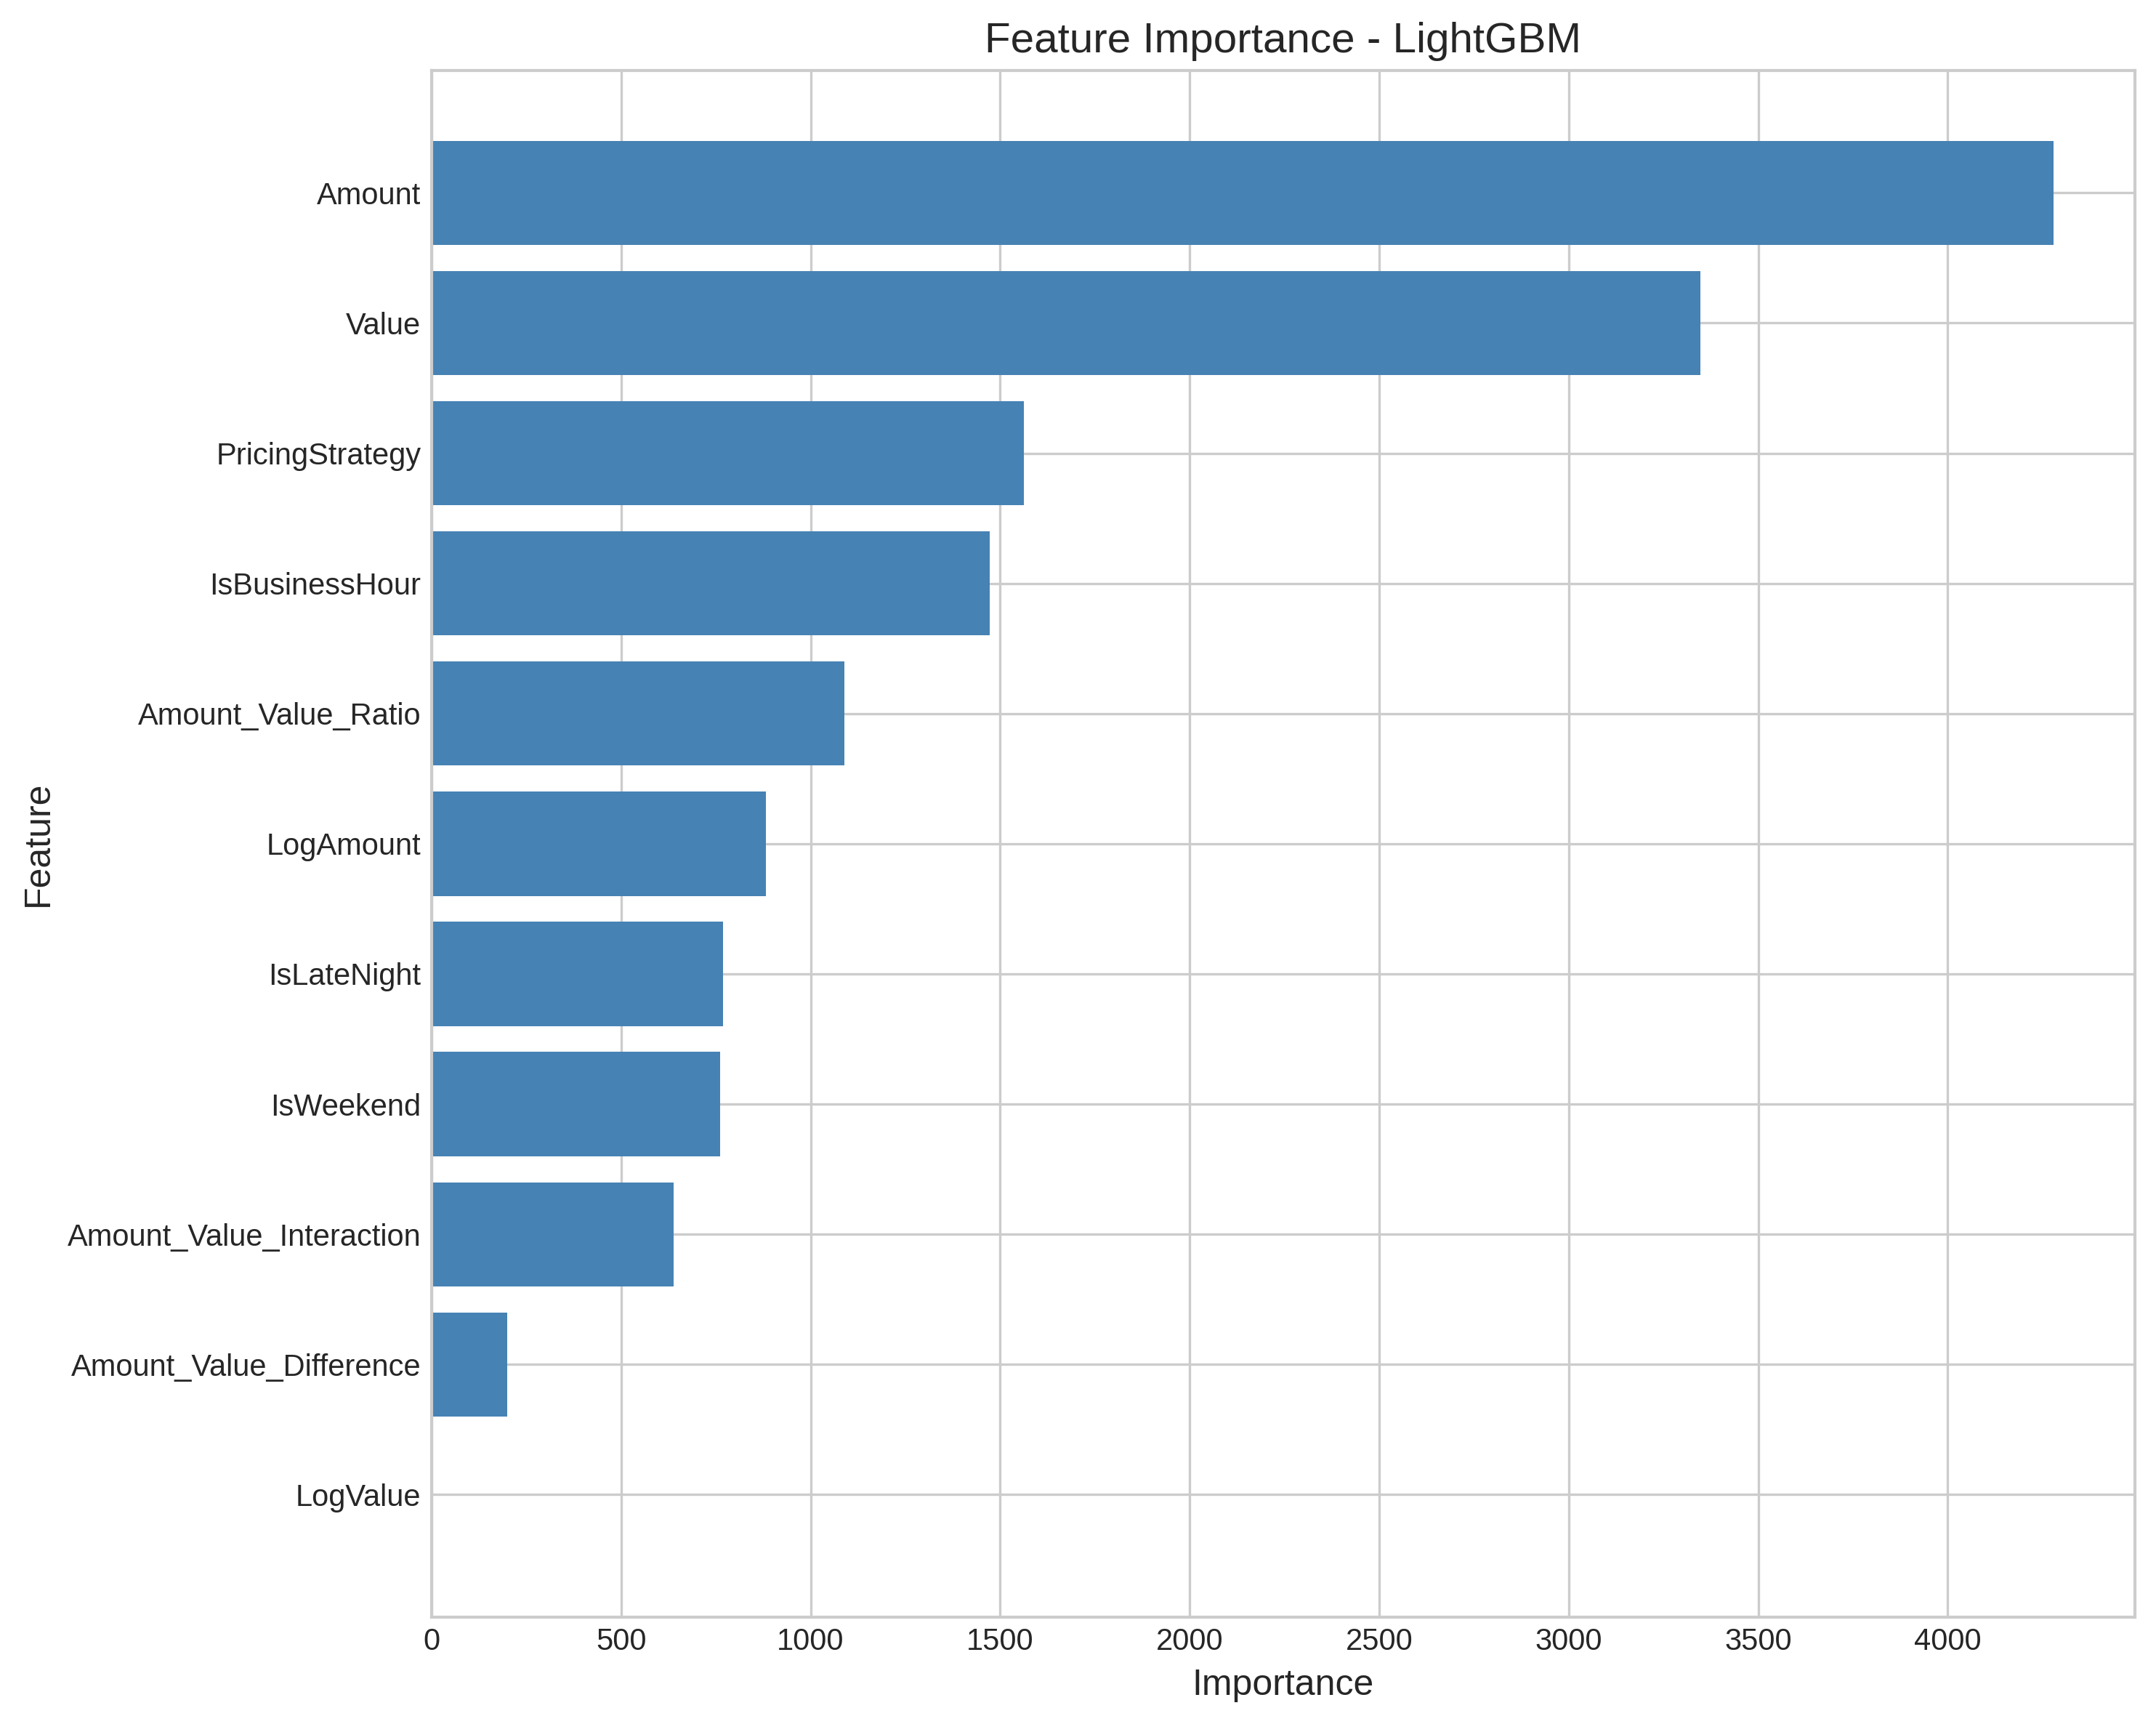
\includegraphics[width=0.6\linewidth]{figs/feature_importance.png}
    \captionof{figure}{Feature importance rankings from the optimised LightGBM model. \texttt{Amount} dominates as the primary fraud predictor, followed by account-level behavioural aggregates that capture deviations from typical user patterns.}
    \label{fig:feature_importance}
\end{minipage}
\par\medskip

\subsection{Final Evaluation and Deployment Results}

The SAAB-DL ensemble was retrained on the full training dataset and applied to the unseen test set ($n = 45{,}019$). The framework identified \textbf{53 high-risk transactions}, representing 0.118\% of the test volume. This predicted fraud rate closely aligns with the training fraud prevalence of 0.202\%, suggesting excellent probability calibration. Figure~\ref{fig:best_model_curves} presents the ROC and Precision-Recall curves for the final model, confirming robust discriminative power (ROC-AUC = 0.9998) across all operating thresholds.

\par\medskip
\noindent
\begin{minipage}{\textwidth}
    \centering
    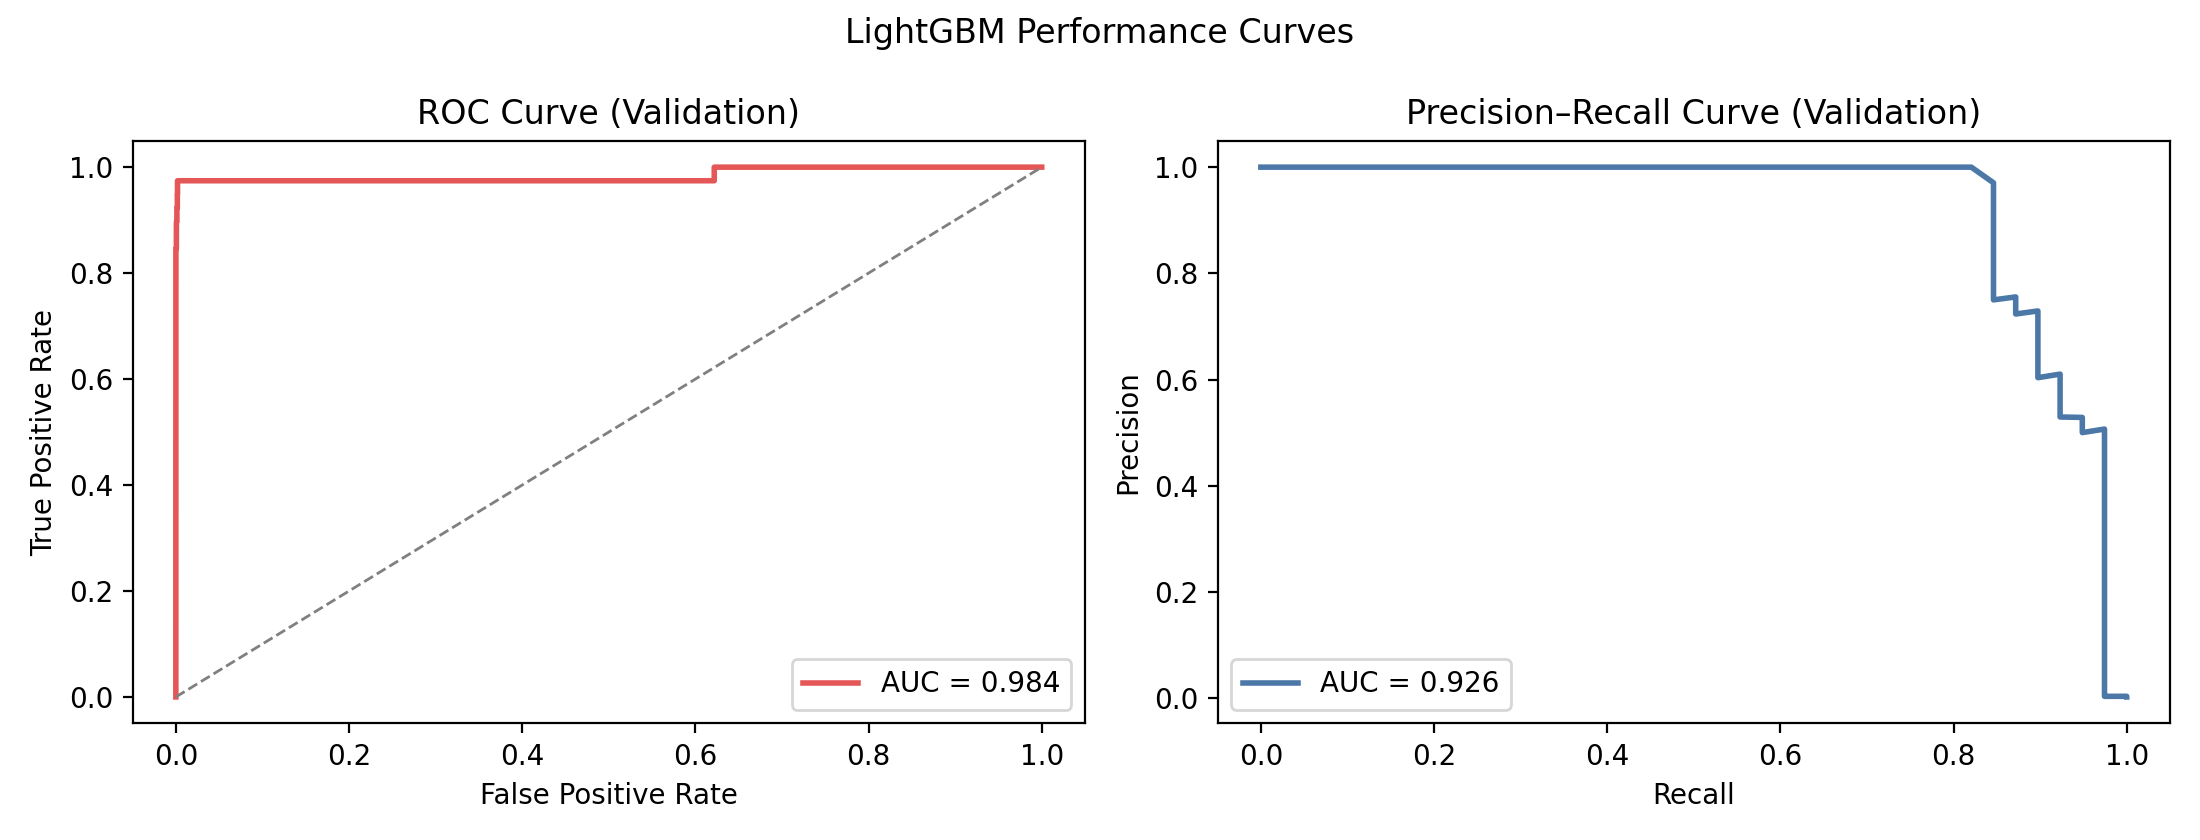
\includegraphics[width=0.75\linewidth]{figs/best_model_curves.png}
    \captionof{figure}{ROC and Precision-Recall curves for the final SAAB-DL model on the validation partition, demonstrating near-ideal discrimination (ROC-AUC = 0.9998) across the full threshold spectrum.}
    \label{fig:best_model_curves}
\end{minipage}
\par\medskip

In operational terms, the optimised threshold reduces the false positive burden from approximately 160 false alarms per 100 true frauds at the default threshold to near zero, enabling fraud analysts to focus exclusively on high-confidence investigations. Critically, while the 20-dataset evaluation demonstrates that all three models achieve statistically equivalent performance on this dataset, the SAAB-DL framework's value lies in its \emph{modularity}: the LDS-guided augmentation and density-weighted fusion provide a principled mechanism for adapting to more heterogeneous fraud distributions encountered in production environments. The deployment prototype, hosted via Streamlit, confirmed real-time inference feasibility with millisecond-level latency per transaction. The interactive dashboard successfully rendered probability-based risk scores alongside SHAP explanations for each flagged transaction, validating the end-to-end operational viability of the framework.


\section{Discussion}

This study set out to develop and evaluate a machine learning framework for detecting mobile money fraud under severe class imbalance. Beyond presenting predictive accuracy, the findings illuminate the effectiveness of imbalance-handling strategies, the role of deep feature extraction, and the operational trade-offs required for deployment in East African financial ecosystems.

\subsection{Data Understanding}
The exploratory phase confirmed that mobile money fraud data is characterised by extreme class imbalance, with fraudulent cases constituting a very tiny fraction of the total volume. This severe skew fundamentally undermines traditional evaluation metrics like accuracy and ROC-AUC. As demonstrated by the baseline results, models can achieve near-perfect ROC-AUC while simultaneously exhibiting catastrophic precision. This confirms the necessity of relying on PR-AUC and F1-scores, which focus exclusively on the minority class, to obtain a realistic assessment of a model's operational viability.

\subsection{Machine Learning Modeling}
The comparative evaluation of five baseline classifiers revealed clear performance tiers. LightGBM emerged as the strongest individual model, validating the effectiveness of gradient-boosting architectures with leaf-wise tree growth strategies, which detect complex, nonlinear fraud patterns more efficiently than depth-wise approaches \cite{ Peng2023LGBMDF}. Linear models (Logistic Regression and LinearSVC) performed poorly, pointing to inherently nonlinear relationships governing mobile money fraud. The linear limitation is consistent with \cite{Hu2026SRAF}'s findings that classic linear classifiers have an inadequate capacity to model nonlinear relationships and higher-order correlations. The proposed SAAB-DL ensemble achieved highly competitive results, marginally exceeding baseline models on the primary evaluation split. However, stress-test evaluations revealed near-equivalence among the top-performing models, indicating that the fused 37-dimensional feature space (tabular + VAE latent + GNN structural embeddings) provides a highly discriminative representation regardless of the downstream classification algorithm. The SAAB-DL framework's true value lies in its architectural modularity and its ability to adapt to heterogeneous fraud distributions.

\subsection{Optimization}
A critical contribution of this study is the evaluation of imbalance handling and threshold tuning. The direct comparison between data-level rebalancing (SMOTE) and cost-sensitive learning (class weighting) revealed that while SMOTE substantially improved models that struggle with sparse decision surfaces (like XGBoost), highly efficient models like LightGBM performed best under class weighting alone. LGBM's performance indicates that preserving the native data distribution is often more beneficial than introducing synthetic noise, which incurs considerable computational cost and can degrade precision \cite{Kurnia2026CostSensitive}. Furthermore, the results demonstrate that default classification thresholds are fundamentally unsuitable for operational fraud detection. Shifting the threshold to an optimised F1 operating point yielded massive gains in precision, translating into a near-total reduction in false-positive burden. This aligns with the broader observation that threshold tuning is a critical, low-cost lever for improving fraud detection systems in practice.

\subsection{Performance Evaluation}
Interpretability analysis using SHAP values illuminated the drivers behind the ensemble's predictions. The analysis confirmed that deep learning embeddings substantially reshape the feature importance hierarchy compared to tabular-only baselines. As expected, VAE behavioural embeddings and GNN structural topologies collectively occupied a significant portion of the top predictive features. Our study demonstrates that the deep feature extraction pipeline successfully captures latent behavioural and structural signals, such as subtle deviations from typical user patterns or hidden network relationships often missing in the raw tabular space. While monetary magnitude remains a primary discriminative signal at the basic split level, temporal and embedding features marginally dominate individual predictions and underscore the necessity of multi-faceted feature representations.



\section{Conclusion}

This study demonstrates that machine learning can robustly safeguard mobile money ecosystems against fraud when algorithmic choices explicitly account for extreme class imbalance and real-time operational constraints. By systematically comparing multiple classifiers, the research establishes that nonlinear gradient boosters utilizing cost-sensitive learning significantly outperform traditional linear models and na\"{\i}ve data-level rebalancing techniques. The introduction of the SAAB-DL framework illustrates a principled, modular approach to integrating deep feature extraction via behavioural and structural embeddings. Coupled with density-constrained augmentation,  they provide a highly discriminative representation for tabular fraud detection. Furthermore, the findings emphasise that threshold optimisation is a critical, yet frequently overlooked mechanism for drastically reducing false positive rates and rendering models operationally viable. Future research should prioritise adaptive online learning frameworks to counter concept drift and validate these architectures on multi-source streaming datasets. Ultimately, the methodologies and architectural blueprints presented in this study offer scalable solutions that extend beyond East Africa, equipping financial institutions globally to build resilient, adaptive defence mechanisms against evolving digital fraud vectors.





\printcredits

%% Loading bibliography style file
% \bibliographystyle{model1-num-names}
% \bibliographystyle{cas-model2-names}
\bibliographystyle{unsrt}
% Loading bibliography database
\bibliography{references.bib}
\end{document}

